\chapter{Johdanto lukuteoriaan}

Kurssin loppuosassa perehdytään lukuteoriaan. Lukuteoria on matematiikan ala, joka tutkii kokonaislukuja. Lukuteorialla on nykyään paljon sovelluksia mm. tietotekniikassa ja digitaalisessa tiedonsiirrossa. Esimerkiksi yleisesti käytetty RSA-sala\-kir\-joi\-tus\-me\-ne\-tel\-mä perustuu lukuteorian tuloksiin. Lukuteoria tarjoaa myös havainnollisen johdannon moniin matemaattisiin ajattelutapoihin, joita käytetään myös muiden matemaattisten teorioiden yhteydessä.

%{\bf Kuva: pankkiautomaatti.}
\begin{center}
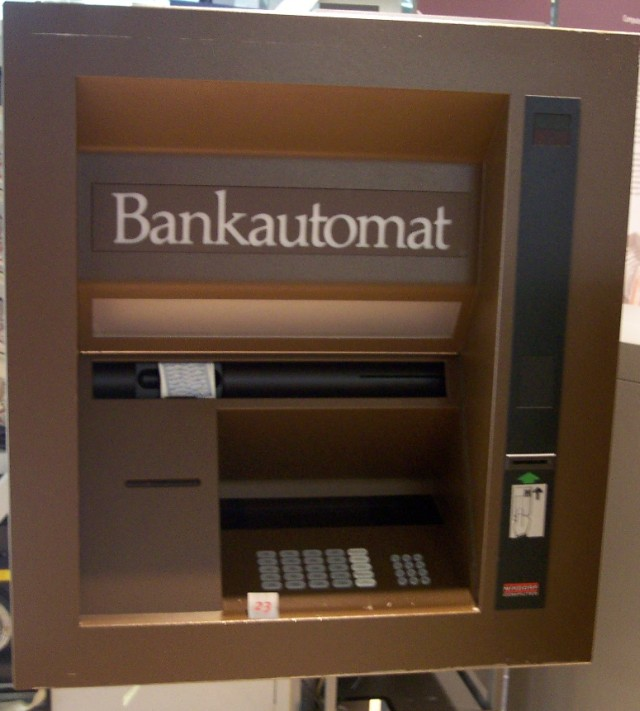
\includegraphics[width=7cm]{pictures/kuvitus/Bankautomat}
\end{center}


\section{Jaollisuus ja jakojäännös}
\label{jaollisuus}
Kokonaislukujen jaollisuus on lukuteoriassa keskeinen käsite, johon on tutustuttu jo alakoulussa.

\subsection*{Tutkimustehtävä} %Palautetaan mieliin jaollisuus ja jakojäännös.
\begin{enumerate}
\item
Laske jakokulmassa a) $905 / 11$ b) $540 / 12$. Ilmoita jakolaskun tulos kokonaisosan ja jakojäännöksen avulla.
\item
Kirjoita kummankin jakolaskun perusteella yhtälö, joka kertoo, kuinka jaettava saadaan
ilmaistua osamäärän, jakajan ja jakojäännöksen avulla.
\end{enumerate}


Alakoulun matematiikassa esimerkiksi kokonaislukujen jakolasku $17/3$ ratkaistaan seuraavasti: $17/3 = 5$, jää $2$. Tämä tarkoittaa, että luku $3$ menee $5$ kertaa lukuun $17$ ja jää $2$. Yleisesti kokonaislukujen $a$ ja $b \neq 0$ jakolaskusta $a/b$ saadaan tulokseksi \termi{osamäärä}{osamäärä} ja \termi{jakojäännös}{jakojäännös}. Edellisessä jakolaskussa osamäärä on $5$ ja jakojäännös on $2$. Mikäli jakojäännös on nolla eli jako menee tasan, sanotaan, että luku $a$ on \termi{jaollisuus}{jaollinen} luvulla $b$ tai että luku $b$ \termi{jaollisuus}{jakaa} luvun $a$. Tällöin merkitään $b|a$. Jos $b|a$, niin luku $a$ voidaan kirjoittaa osamäärän $q$ ja luvun $b$ avulla $a = qb$. Itse asiassa nämä ehdot ovat yhtäpitäviä. Jos luku $a$ ei ole jaollinen luvulla $b$, merkitään $b \nmid a$.

\begin{esimerkki}
%{\bf Esimerkki 1.}
 Tutki, onko totta, että a)  $3 | 6$  b)  $2 | 5$ c) $-4|12$.

{\bf Ratkaisu:}

a) Tapa 1: Suoritetaan jakolasku $6/3= 2$. Jako menee tasan, joten luku $6$ on jaollinen luvulla $3$. Siis $3 | 6$.

Tapa 2: Koska $6 = 2 \cdot 3$, luku $3$ on luvun $6$ tekijä. Siis $3 | 6$.

b) Tapa 1: Suoritetaan jakolasku $5/2 = 2$, jää $1$. Jako ei mene tasan, joten luku $5$ ei ole jaollinen luvulla $2$. Siis $2 \nmid 5$.

Tapa 2: Lukua $5$ ei voida kirjoittaa muodossa $2q$, missä $q\in\Z$, sillä luku $5$ ei ole parillinen. Siis $2 \nmid 5$.

c) 
Tapa 1: Suoritetaan jakolasku $12/(-4)=-12/4= -3$. Jako menee tasan, joten luku $12$ on jaollinen luvulla $-4$. Siis $-4 | 12$.

Tapa 2: Koska $12 = -3 \cdot (-4)$, luku $-4$ on luvun $12$ tekijä. Siis $-4 | 12$.

{\bf Vastaus:} a) On.  b) Ei ole. c) On.
\end{esimerkki}

Jaollisuuden tutkimisessa tärkeä tulos on seuraava lause, jonka todistus on melko vaativa:

\laatikko{
{\bf Lause (Jakoyhtälö).}
Jos $a$ ja $b$ ovat kokonaislukuja ja $b > 0$, niin on\newline olemassa sellaiset
 yksikäsitteiset kokonaisluvut $q$ ja $r$, että
\[
a = qb + r,\qquad 0\le r<b.
\]
}

Jakoyhtälössä esiintyvää lukua $q$ sanotaan lukujen $a$ ja $b$ (vaillinaiseksi) osamääräksi ja lukua $r$  jakojäännökseksi.

%Jakojäännökselle käytetään myös merkintää 
%\[
%r = a \mod b.
%\]

\begin{todistus}% (Lisämateriaali)
Todistetaan väite tapauksessa $a\ge 0$. Tutkitaan aluksi joukkoja
\[
S = \{ a-nb\,|\, n\in \Z\}.
\]
Koska $a\in S$, tässä joukossa on ainakin yksi epänegatiivinen alkio. Olkoon $r=a-qb$ joukon $S$ pienin epänegatiivinen alkio. Nyt $r < b$, koska muuten luku 
\[
0\le r - b = a - qb - b = a - (q+1)b 
\]
olisi lukua $r$ pienempi joukon $S$ epänegatiivinen alkio.

Yksikäsitteisyyden toteamiseksi tehdään vastaoletus, että
\[
a= q_1b+r_1 = q_2b+r_2.
\]
Voidaan olettaa, että $q_2>q_1$. Nyt
\[
r_1 - r_2 = q_2b - q_1b = (q_2-q_1)b \ge b.
\]
Toisaalta $r_1-r_2<b$, koska $0\le r_1 < b$ ja $0\le r_2 < b$, mikä on ristiriita. Siten ainoa mahdollisuus on, että $q_1=q_2$ ja $r_1=r_2$. 
\end{todistus}

\begin{esimerkki}
%{\bf Esimerkki 2.}
%Määritä jakolaskun $a/b$ osamäärä ja jakojäännös, kun
%a) $a=23$ ja $b=5$, 
%b) $a=-19$ ja $b=6$. 
%Kirjoita vastaavat jakoyhtälöt.
Määritä jakolaskun osamäärä ja jakojäännös sekä kirjoita vastaava jakoyhtälö, kun
a) luku $23$ jaetaan luvulla $5$,  b)  luku $-19$ jaetaan luvulla $6$.

{\bf Ratkaisu:}
a) Vaillinainen osamäärä voidaan selvittää päässälaskulla tai laskinta käyttäen. Laskinta käytettäessä lasketaan jakolasku normaalisti ja otetaan lopputuloksen kokonaisosa.

Laskin antaa $23/5 = 4,6$, joten vaillinaiseksi osamääräksi saadaan $4$.

Jakojäännös saadaan nyt selville vähentämällä luku $4\cdot 5$ jaettavasta $23$, siis $23-4\cdot 5=3$. Siten jakojäännökseksi saadaan $3$. 
%Voidaan myös merkitä
%\[
%r=23 \mod 5 = 3.
%\]
Jakoyhtälö on
\[
23 = 4\cdot 5 + 3.
\]

b) Laskin antaa $-19/6 \approx -3,167$. Vaillinaiseksi osamääräksi on valittava $-4$, jotta jakojäännös olisi epänegatiivinen.

Jakojäännös saadaan jälleen selville vähentämällä luku $-4\cdot 6$ jaettavasta $-19$, siis $-19-(-4)\cdot 6=-19+24=5$. Siten jakojäännökseksi saadaan $5$. 
Jakoyhtälö on
\[
-19 = -4\cdot 6 +5.
\]

{\bf Vastaus:} a) $23 = 4\cdot 5 + 3$, b) $-19 = -4\cdot 6 +5$.
\end{esimerkki}

\bigskip

\begin{center}
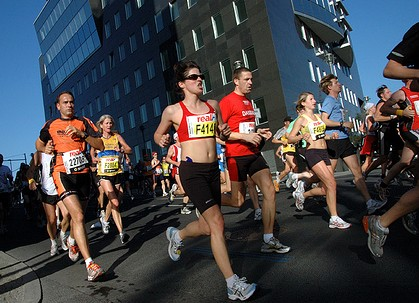
\includegraphics[width=10cm]{pictures/kuvitus/Berlin_marathon}
\end{center}


\begin{esimerkki}
%{\bf Esimerkki 3.} %Anna-Maija keksii konkreettisen / soveltavan esimerkin. 
Jussi tavoittelee Cooperin testissä tulosta 3050 metriä. Testi juostaan 400 metriä pitkällä
radalla. Kuinka monta kokonaista kierrosta Jussin pitää juosta? Kuinka pitkä matka
hänen pitää juosta vielä kokonaisten kierrosten lisäksi?

{\bf Ratkaisu:}
Jaetaan ensin tavoiteltava tulos yhden ratakierroksen pituudella:
$3050  / 400  = 7,625$. Jussin pitää siis juosta $7$ kokonaista kierrosta.
Koska $3050  - 7 \cdot 400 = 3050  - 2800  = 250$, Jussin pitää juosta kokonaisten kierrosten lisäksi $250$ metriä.

{\bf Vastaus:} Jussin on juostava $7$ kokonaista kierrosta ja $250$ metriä.
\end{esimerkki}

\begin{esimerkki}
%{\bf Esimerkki 4.}
Olkoot $a$, $b$ ja $c$ kokonaislukuja ja $a\neq 0$. Osoita, että jos $a|b$ ja $a|c$, niin $a|(b + c)$.

{\bf Ratkaisu:}
Jos $a|b$, niin on olemassa sellainen kokonaisluku $q$, että $b = qa$.
Jos $a|c$, niin on olemassa sellainen kokonaisluku $r$, että $c = ra$.
Tällöin $b + c = qa + ra = (q + r)a$, missä $q + r$ on kokonaisluku. 
Siis $a|(b + c)$.
\end{esimerkki}

%\newpage

%\section*{Tehtäviä}

\Harjoitustehtavat

\begin{enumerate}

\item Onko luku a) $50$ b) $48$ c) $-72$ d) $-34$ jaollinen luvulla $6$?

\item Jakaako luku $13$ luvun a) $117$ b) $-65$ c) $160$ d) $-81$?

\item Osoita, että a) $3|66$ b) $7\nmid 120$ c) $15|(-330)$ d) $11\nmid (-619)$.

\item Onko väite tosi? a) $3|53$ b) $-9|108$ c) $12 \nmid (-158)$ d) $-7|175$ e) $-17 \nmid (-646)$

\item Kirjoita jakoyhtälö, kun
\begin{itemize}
\item[a)] luku $7$ jaetaan luvulla $3$
\item[b)] luku $51$ jaetaan luvulla $4$
\item[c)] luku $1000$ jaetaan luvulla $125$
\item[d)] luku $3858$ jaetaan luvulla $97$.
\end{itemize}

\item Kirjoita jakoyhtälö, kun
\begin{itemize}
\item[a)] luku $-22$ jaetaan luvulla $7$
\item[b)] luku $-2844$ jaetaan luvulla $36$
\item[c)] luku $-3858$ jaetaan luvulla $97$.
\end{itemize}

\item Kirjoita jakoyhtälö jakolaskulle a) $9/25$ b) $-9/25$ c) $124/120$ d) $-124/120$.

\item Päättele, mikä on jakojäännös, kun
\begin{itemize}
\item[a)] luku $1967$ jaetaan luvulla $5$
\item[b)] luku $-426$ jaetaan luvulla $5$
\item[c)] luku $67876$ jaetaan luvulla $50$
\item[d)] luku $-30509$ jaetaan luvulla $50$.
\end{itemize}

\item Leipomossa on pakattavana $260$ sämpylää. Kuinka monta täyttä pussia saadaan ja kuinka monta sämpylää jää yli, jos käytetään vain a) $24$ b) $10$ c) $6$ d) $4$ sämpylän pusseja?

\item 
Jos kello on nyt 13.05, niin mitä kello oli 2012 tuntia ja 45 minuuttia sitten?

\item 
\begin{itemize}
\item[a)] Mikä luku jaettuna luvulla $17$ antaa osamääräksi $98$ ja jakojäännökseksi $5$?
\item[b)] Mikä luku jaettuna luvulla $12$ antaa osamääräksi $-91$ ja jakojäännökseksi $0$?
\item[c)] Millä positiivisella kokonaisluvulla luku $146$ on jaettava, jotta osamäärä olisi $3$ ja jakojäännös $2$?
\item[d)] Millä positiivisella kokonaisluvulla luku $72$ on jaettava, jotta jakojäännös olisi 7?
\end{itemize}

\item Määritä osamäärä ja jakojäännös sekä kirjoita jakoyhtälö, kun a) luku $2^{18} + 10$ jaetaan luvulla $2^{15} + 1$ b) luku $3^{100} + 100$ jaetaan luvulla $3^{98} + 10$.

\item Olkoot $a$, $b$, $c$, $r$ ja $s$ kokonaislukuja ja $a \neq 0$. Osoita, että jos $a|b$ ja $a|c$, niin $a|(rb + sc)$.

\item Olkoot $a$, $b$, $c$ ja $d$ kokonaislukuja ja $a,b \neq 0$. Osoita, että jos $a|c$ ja $b|d$, niin $(ab)|(cd)$.

\item Osoita, että jos $a$ ja $b$ ovat parittomia kokonaislukuja, niin $4 | (a^2 - b^2)$.

\item Olkoot $a$ ja $b$ nollasta eroavia kokonaislukuja. Mitä voidaan päätellä, jos $a|b$ ja $b|a$?

\item Olkoon $n$ positiivinen kokonaisluku. Määritä osamäärä ja jakojäännös sekä kirjoita jakoyhtälö, kun
\begin{itemize}
\item[a)] luku $5n + 3$ jaetaan luvulla $5$
\item[b)] luku $n^2 + 2n + 2$ jaetaan luvulla $n + 1$
\item[c)] luku $n^3 + 3n^2 - n - 3$ jaetaan luvulla $n + 3$
\item[d)] luku $2n^3 + 3n^2 + 4n + 9$ jaetaan luvulla $2n + 3$.
\end{itemize}

\item
\begin{itemize}
\item[a)] Muodosta jakoyhtälö luvuille $0,1,2,\ldots,7$, kun jakajana on luku $3$. Mitä arvoja jakojäännös voi saada?
\item[b)] Osoita, että jos kahden kokonaisluvun tulo on jaollinen luvulla $3$, niin ainakin toinen luvuista on jaollinen luvulla $3$. Vihje: Käytä epäsuoraa todistusta.
\end{itemize}

\end{enumerate}

\subsection*{Kotitehtäviä}

\begin{enumerate}

\item Onko luku a) $42$ b) $-75$ c) $102$ d) $-98$ jaollinen luvulla $7$?

\item Jakaako luku $11$ luvun a) $-165$ b) $21$ c) $-101$ d) $209$?

\item Osoita, että a) $2|234$ b) $-17|408$ c) $14 \nmid 223$ d) $6 \nmid (-472)$.

\item Onko väite tosi? a) $8 \nmid 168$ b) $13 \nmid (-95)$ c) $-5|777$ d) $29\nmid 2583$ e) $-4|(-924)$

\item Kirjoita jakoyhtälö, kun
\begin{itemize}
\item[a)] luku $9$ jaetaan luvulla $6$
\item[b)] luku $576$ jaetaan luvulla $19$
\item[c)] luku $3712$ jaetaan luvulla $32$.
\end{itemize}

\item Kirjoita jakoyhtälö, kun
\begin{itemize}
\item[a)] luku $-12$ jaetaan luvulla $5$
\item[b)] luku $-147$ jaetaan luvulla $6$
\item[c)] luku $-875$ jaetaan luvulla $35$.
\end{itemize}

\item Kirjoita jakoyhtälö jakolaskulle a) $3/17$ b) $-3/17$ c) $88/80$ d) $-88/80$.

\item Päättele, mikä on jakojäännös, kun
\begin{itemize}
\item[a)] luku $5555$ jaetaan luvulla $4$
\item[b)] luku $-555$ jaetaan luvulla $4$
\item[c)] luku $123456$ jaetaan luvulla $100$
\item[d)] luku $-654321$ jaetaan luvulla $100$.
\end{itemize}

\item Tänään on keskiviikko. Mikä viikonpäivä a) on 1000 päivän kuluttua b) oli 500 päivää sitten?

\item Kello on $17.28$ ja on tiistai. Mitä kello on 2073 tunnin kuluttua? Mikä viikonpäivä silloin on?

\item Tarkastellaan kirjainjonoa ABCDEFGABCDEFGABCDEFG... a) Mikä on jonon 12742. kirjain? b) Kuinka monta A-kirjainta on jonossa ennen sitä?

\item 
\begin{itemize}
\item[a)] Mikä luku jaettuna luvulla $19$ antaa osamääräksi $6$ ja jakojäännökseksi $13$?
\item[b)] Mikä luku jaettuna luvulla $7$ antaa osamääräksi $-23$ ja jakojäännökseksi $5$?
\item[c)] Millä positiivisella kokonaisluvulla luku $1263$ on jaettava, jotta osamäärä olisi $114$ ja jakojäännös $9$?
\item[d)]  Millä positiivisella kokonaisluvulla luku $-140$ on jaettava, jotta jakojäännös olisi $3$?
\end{itemize}

\item Olkoon $n$ kokonaisluku. Osoita, että luku $(3n+1)^4 - (3n+1)^3$ on jaollinen luvulla 3. Vihje: Käytä symbolisen laskimen {\tt expand}-toimintoa.

\item Olkoon $n$ kokonaisluku. Osoita, että luku $(2n+1)^5 - (2n-1)^4-2n$ on jaollinen luvulla $16$.

\item Määritä osamäärä ja jakojäännös sekä kirjoita jakoyhtälö, kun a) luku $7^{50} + 1$ jaetaan luvulla $7^{48} - 1$ b) luku $7^{50} - 1$ jaetaan luvulla $7^{25} + 1$.

\item Olkoot $a$, $b$ ja $c$ kokonaislukuja ja $a \neq 0$. Osoita, että jos $a|b$ ja $a|(b + c)$, niin $a|c$.

\item Olkoot $p$, $q$ ja $r$ positiivisia kokonaislukuja. Osoita, että jos $p$ on luvun $q$ tekijä ja $q$ on luvun $r$ tekijä, niin $p$ on luvun $r$ tekijä.

\item Olkoot $a$, $b$ ja $c$ kokonaislukuja ja $a,c \neq 0$. Osoita, että jos $(ac)|(bc)$, niin $a|b$.

\item Olkoot $a$ ja $b$ kokonaislukuja. Osoita, että luku $a + b$ on jaollinen luvulla $3$ silloin ja vain silloin, kun luku $a - 2b$ on jaollinen luvulla $3$.

\item Olkoon $n$ positiivinen kokonaisluku. Määritä osamäärä ja jakojäännös sekä kirjoita jakoyhtälö, kun
\begin{itemize}
\item[a)] luku $2n^2 - n - 2$ jaetaan luvulla $n + 1$
\item[b)] luku $n^3 + n^2 + 6$ jaetaan luvulla $n + 2$
\item[c)] luku $n^2 + 2n - 1$ jaetaan luvulla $n$.
\end{itemize}
Vihje: Voit laskea polynomien jakolaskun symbolisen laskimen avulla.

\item * %(Lisämateriaalia.)
Todista jakoyhtälö, kun $a<0$.

\item *
%(Lisämateriaalia.) 
\termi{lukujärjestelmä}{Lukujärjestelmä} tarkoittaa tapaa, jolla luvut kirjoitetaan numeroiden avulla. \termi{kantaluku}{Kantaluku} kertoo, kuinka monta eri numeroa lukujärjestelmän luvuissa voi esiintyä. Esimerkiksi \termi{kymmenjärjestelmä}{kymmenjärjestelmässä} kantaluku on $10$ ja käytössä ovat numerot $0,1,2,3,4,5,6,7,8$ ja $9$. Kymmenjärjestelmän luku $3258$ muodostuu numeroista $3,2,5$ ja $8$ kantaluvun $10$ potenssien avulla seuraavasti:
\begin{eqnarray*}
3258 &=&3\cdot 1000+2\cdot 100+5\cdot 10+8\\
&=& 3\cdot 10^3+2\cdot 10^2+5\cdot 10^1+8\cdot 10^0.
\end{eqnarray*}
Kymmenjärjestelmässä siis luvun viimeinen numero on luvun $10^0$ kerroin, toiseksi viimeinen luvun $10^1$ kerroin, kolmanneksi viimeinen luvun $10^2$ kerroin jne.

\termi{kaksijärjestelmä}{Kaksijärjestelmän} eli \termi{binäärijärjestelmä}{binäärijärjestelmän} luvut taas muodostuvat numeroista $0$ ja $1$. Esimerkiksi binääriluku $101101$ voidaan ilmaista kymmenjärjestelmässä kirjoittamalla luku kantaluvun $2$ potenssien avulla seuraavasti:
\begin{eqnarray*}
101101&=&1\cdot2^5+0\cdot2^4+1\cdot2^3+1\cdot2^2+0\cdot2^1+1\cdot2^0 \\
&=& 1\cdot32+0\cdot16+1\cdot8+1\cdot4+0\cdot2+1=45.
\end{eqnarray*}

Kaksijärjestelmässä siis luvun viimeinen numero on luvun $2^0$ kerroin, toiseksi viimeinen luvun $2^1$ kerroin, kolmanneksi viimeinen luvun $2^2$ kerroin jne.

Kymmenjärjestelmän lukuja voidaan muuntaa binääriluvuiksi jakoyhtälöiden avulla. Muunnetaan luku 18 binääriluvuksi. Jaetaan ensin kymmenjärjestelmän luku 18 kaksijärjestelmään kantaluvulla 2 ja kirjataan ylös jakojäännös. Tämän jälkeen jaetaan edellisen jakolaskun osamäärä kantaluvulla 2 ja kirjataan taas jakojäännös muistiin. Näin jatketaan, kunnes osamääräksi jää luku 0. 
\begin{eqnarray*}
18&=&9\cdot 2+0\\
9&=&4\cdot 2+1\\
4&=&2\cdot 2+0\\
2&=&1\cdot 2+0\\
1&=&0\cdot2+1 \to \textrm{lopetetaan}
\end{eqnarray*}
Kirjoittamalla nyt jakojäännökset lopusta alkuun saadaan luku $10010$. Se on kymmenjärjestelmän luvun $18$ binääriesitys.
\begin{itemize}
\item[a)] Muunna binäärijärjestelmän luvut $1001$ ja $110110100$ kymmenjärjestelmään.
\item[b)] Muunna kymmenjärjestelmän luvut $25$ ja $520$ binäärijärjestelmään.
\item[c)] Etsi laskimesi ohjekirjasta, miten muunnokset voidaan toteuttaa laskimella.
\item[d)] Ohjelmoi laskimesi ohjelmointikielellä ohjelma, joka suorittaa muunnoksen kymmenjärjestelmästä binäärijärjestelmään.
\end{itemize}

\end{enumerate}




\newpage


\section{Kongruenssi} 
Luonnonilmiöitä mallinnettaessa tulee usein vastaan tilanteita, joissa on hyödyllistä samastaa keskenään jaksollisesti toistuvat ilmiöt. Tällaisia ilmiöitä ovat esimerkiksi vuodenajat, viikonpäivät ja kellonajat. Samaan tapaan kokonaislukujen jonossa esimerkiksi parilliset tai yhdellätoista jaolliset luvut esiintyvät jaksollisesti. Lukujonossa toistuvien ominaisuuksien tutkimisessa käytetään \termi{kongruenssi}{kongruenssin} käsitettä.

\subsection*{Tutkimustehtävä}
\begin{enumerate}
\item Ryhmittele luvut $16$, $59$, $12$, $3$, $177$, $21$, $47$, $65$, $222$, $-17$, $-100$ ja $-1$ niin, että samaan joukkoon kuuluvat ne luvut, joilla on sama jakojäännös, kun ne jaetaan luvulla $5$.
\item Valitse ensin kaksi lukua, jotka ovat samassa kohdan 1 joukossa. Laske niiden erotus. Toista kaksi kertaa. Valitse sitten kaksi lukua, jotka ovat eri joukoissa kohdassa 1. Laske niiden erotus. Toista kaksi kertaa. Miten erotuksen arvosta näkee, kuuluvatko vähenevä ja vähentäjä samaan kohdan 1 joukkoon?
\item Miten voit esittää yleisessä muodossa kaikki ne kokonaisluvut, jotka ovat jaollisia luvulla $5$? Entä ne luvut, joiden jakojäännös on $1, 2, 3$ tai $4$, kun jaetaan luvulla $5$?
\item Todista kohdan 2 havaintosi.
\end{enumerate}

Kokonaislukujen $a$ ja $b$ kongruenssi tarkoittaa, että niillä on sama jakojäännös jaettaessa positiivisella kokonaisluvulla $k$. Kongruenssille on käytännöllistä antaa seuraava matemaattinen määritelmä.

%---
%{\bf Teorialaatikko [Kongruenssi].}

%\fbox{
%\begin{minipage}{12cm}
\laatikko{
{\bf Kongruenssi.}
%\medskip
Kokonaisluvut $a$ ja $b$ ovat \termi{kongruentti modulo $k$}{kongruentteja modulo} $k$, jos erotus\newline
 $a-b$ on jaollinen positiivisella kokonaisluvulla $k$. Tällöin merkitään
\[
a \equiv b \quad (\mod k).
\]
%, eli \[ a \mod k = b \mod k.\]
Jos $a$ ja $b$ eivät ole kongruentteja modulo $k$, merkitään
\[
a \not\equiv b \quad (\mod k).
\]
Merkintää $(\mod k)$ ei ole tapana kirjoittaa, jos luku $k$ on asiayhteydestä selvä.
%\end{minipage}
%---
}

Kongruenssiyhtälön
\[
a\equiv b\qquad (\mod k)
\]
kanssa on yhtäpitävää, että $a-b=nk$ eli $a=b+nk$ vähintään yhdellä luvulla $n\in \Z$.


%{\bf Esimerkki 1.} 
\begin{esimerkki}
Osoita, että a) $27 \equiv 19 \ (\mod 4)$ b) $13 \equiv -82 \ (\mod 5)$.

{\bf Ratkaisu:}

a) Tapa 1

Koska $27 - 19 = 8 = 2\cdot 4$, niin erotus $27-19$ on jaollinen luvulla $4$. Siten $27 \equiv 19 \ (\mod 4)$.

Tapa 2

Kun luku $27$ jaetaan luvulla $4$, saadaan jakoyhtälö $27 = 6 \cdot 4 + 3$. Vastaavasti $19 = 4 \cdot 4 + 3$. Luvuilla $27$ ja $19$ on siis sama jakojäännös, $3$, kun jaetaan luvulla $4$. Siten $27 \equiv 19\ (\mod 4)$.

b) Koska $13 - (-82) = 95 = 19 \cdot 5$, niin $5 | (13 - (-82))$. Siten $13 \equiv -82 \ (\mod 5)$.


{\bf Esimerkki 2.}
Hannalla on kaksi lasta, Aaro ja Mirkku. Hanna laski, että Aaron syntymäpäivä on 38 päivän kuluttua  ja Mirkun 59 päivän kuluttua äidin syntymäpäivästä. Ovatko Aaron ja Mirkun syntymäpäivät samana viikonpäivänä?

{\bf Ratkaisu:}
Tutkitaan, ovatko luvut $38$ ja $59$ kongruentteja modulo $7$. Koska $59 - 38 = 21 = 3\cdot 7$, niin $59 \equiv 38\ (\mod 7)$. Aaron ja Mirkun syntymäpäivät ovat siis  samana viikonpäivänä.

{\bf Vastaus:} Ovat.
\end{esimerkki}

\begin{esimerkki}
%{\bf Esimerkki 3.} 
\begin{itemize}
\item[a)] Määritä pienin epänegatiivinen kokonaisluku, joka on kongruentti luvun $45$ kanssa modulo $7$.
\item[b)] Jos tänään on perjantai ja loman alkuun on $45$ päivää, niin minä viikonpäivänä loma alkaa?
\end{itemize}

{\bf Ratkaisu:}

a)
Kun luku $45$ jaetaan luvulla $7$, saadaan jakoyhtälö $45 = 6 \cdot 7 + 3$. Koska voidaan kirjoittaa $45 - 3 = 6 \cdot 7$, nähdään, että jakojäännös $3$ on kongruentti luvun $45$ kanssa modulo 7. Luku $3$ on myös pienin epänegatiivinen kokonaisluku, joka on kongruentti luvun $45$ kanssa modulo $7$.

b)
a-kohdan perusteella luku $3$ on kongruentti luvun $45$ kanssa modulo $7$. Kysytty viikonpäivä saadaan selville laskemalla perjantaista $3$ päivää eteenpäin, jolloin on maanantai. Siis loma alkaa maanantaina. 

{\bf Vastaus:} a) 3 b) Loma alkaa maanantaina.
\end{esimerkki}

\subsection*{Kongruenssin laskusääntöjä} Kongruensseilla on monia ominaisuuksia, jotka muistuttavat yhtälöiden ratkaisemisessa käytettäviä laskusääntöjä.

\laatikko{
{\bf Lause.} Olkoot $a,b,c,d\in \Z$ ja $k,n \in \Z_+$ sekä $a \equiv c$,\newline
$b \equiv d\quad (\mod k)$. Tällöin:
\begin{enumerate}
\item $a+b\equiv c+d\quad (\mod k)$,
\item $a-b\equiv c-d\quad (\mod k)$,
\item $ab \equiv cd\quad (\mod k)$,
\item $a^n \equiv c^n \quad (\mod k)$.
\end{enumerate}
}

\begin{todistus}
Todistetaan kohdat 1 ja 3. Kohdan 2 todistus on kotitehtävänä, ja potenssisääntö 4 todistetaan lisämateriaalina olevan kappaleen 5.4 tehtävässä XX.

Kongruenssin määritelmän perusteella $a=c + mk$ ja $b= d + nk$, missä $m,n\in \mathbb{Z}$.

Siten
\begin{eqnarray*}
a+b - (c+d) &=& c + mk + d + nk - c - d\\ &=& mk + nk = (m+n)k,
\end{eqnarray*}
missä $(m+n)$ on kokonaisluku. Siis erotus $a + b - (c+d)$ on jaollinen luvulla $k$, joten ensimmäinen väite pätee.

Samaan tapaan saadaan
\begin{eqnarray*}
ab - cd &=& (c + mk)(d + nk) - cd\\ &=& cd +c nk + d mk + mnk^2 - cd\\ &=& (cn+dm+mnk)k,
\end{eqnarray*}
missä $(cn+dm+mnk)$ on kokonaisluku. Siten erotus $ab - cd$ on jaollinen luvulla $k$, joten kolmas väite pätee.
\end{todistus}


Erityisesti tuloksesta seuraa, että  jos $a\equiv b \ (\mod k)$, niin $na\equiv nb
\ (\mod k)$ kaikilla $n\in \Z$.


%{\bf Esimerkki 4.}
\begin{esimerkki}
Määritä pienin epänegatiivinen luku, jonka kanssa luku a) $350 - 7778$, b) $65 \cdot 141$, c) $16^{10} + 82$ on kongruentti modulo $7$.

{\bf Ratkaisu:}

Korvataan luvut mahdollisimman yksinkertaisilla luvuilla, jotka ovat kongruentteja modulo $7$, ja sovelletaan kongruenssin laskusääntöjä.

a)
Koska $350 \equiv 0$ ja $7778 \equiv 1 \ (\mod 7)$, niin säännön 2 mukaan $350 - 7778 \equiv 0 - 1 = -1 \equiv 6 \ (\mod 7)$.

b)
Koska $65 \equiv 2$ ja $141 \equiv 1 \ (\mod 7)$, niin säännön 3 mukaan $65 \cdot 141 \equiv 2 \cdot 1 = 2 \ (\mod 7)$.

c)
Koska $16 \equiv 2$ ja $82 \equiv 5 \ (\mod 7)$, niin säännön 1 ja potenssisäännön 4 mukaan
$16^{10} + 82 \equiv 2^{10} + 5 = 1024 + 5 = 1029 \equiv 0 \ (\mod 7)$.

{\bf Vastaus:} a) $6$ b) $2$ c) $0$
\end{esimerkki}

\begin{esimerkki}
%{\bf Esimerkki 5.}
Osoita, että luku $n^4 + 2n^3 + n^2$ on
jaollinen luvulla $4$, kun $n$ on kokonaisluku.

{\bf Ratkaisu:}
Kun kokonaisluku jaetaan luvulla $4$, jakojäännös voi olla $0$,
$1$, $2$ tai $3$. Siten jokainen kokonaisluku $n$ on jotakin
seuraavaa muotoa: $4q$, $4q + 1$, $4q + 2$ tai $4q + 3$, missä
$q\in\Z$. Tutkitaan luvun $n^4 + 2n^3 + n^2$ jaollisuutta luvulla
$4$ erikseen kussakin näistä osajoukoista.

Tapa 1: Kirjoitetaan lauseke $n^4 + 2n^3 + n^2$ muotoon
\[
n^4 + 2n^3 + n^2 = n^2 (n^2 + 2n + 1) = n^2 (n + 1)^2.
\]

1) Kun $n = 4q$, niin
\begin{eqnarray*}
n^4 + 2n^3 + n^2 &=& (4q)^2(4q + 1)^2 = 4^2 \cdot q^2 (4q + 1)
^2\\
&=& 4 \cdot 4q^2 (4q + 1)^2.
\end{eqnarray*}
Koska $4q^2 (4q + 1)^2 \in \Z$, niin luku $n^4 + 2n^3 + n^2$ on jaollinen luvulla $4$.

2) Kun $n = 4q + 1$, niin
\begin{eqnarray*}
n^4 + 2n^3 + n^2 &=& (4q+1)^2(4q + 2)^2 = (4q+1)^2 (2(2q + 1))
^2\\
&=& (4q+1)^2 \cdot 2^2 \cdot (2q + 1)^2 = 4(4q+1)^2 (2q + 1)^2,
\end{eqnarray*}
joten luku $n^4 + 2n^3 + n^2$ on jaollinen luvulla $4$.

3) Kun $n = 4q + 2$, niin
\begin{eqnarray*}
n^4 + 2n^3 + n^2 &=& (4q+2)^2(4q + 3)^2 = (2(2q+1))^2 (4q + 3)
^2\\
&=& 2^2 \cdot (2q+1)^2 (4q + 3)^2 = 4(2q+1)^2 (4q + 3)^2,
\end{eqnarray*}
joten luku $n^4 + 2n^3 + n^2$ on jaollinen luvulla $4$.

4) Kun $n = 4q + 3$, niin
\begin{eqnarray*}
n^4 + 2n^3 + n^2 &=& (4q+3)^2(4q + 4)^2 = (4q+3)^2 (4(q + 1))^2\\
&=& (4q+3)^2 \cdot 4^2 \cdot (q + 1)^2 = 4(4q+3)^2 \cdot 4 \cdot
(q + 1)^2,
\end{eqnarray*}
joten luku $n^4 + 2n^3 + n^2$ on jaollinen luvulla $4$.

Siis luku $n^4 + 2n^3 + n^2$ on jaollinen luvulla $4$, kun $n$ on
kokonaisluku.

Tapa 2:

1) Kun $n = 4q$, niin $n\equiv0\ (\mod 4)$. Siten
\[
n^4 + 2n^3 + n^2 \equiv 0^4 + 2 \cdot 0^3 + 0^2 = 0\ (\mod 4)
\]
ja luku $n^4 + 2n^3 + n^2$ on jaollinen luvulla $4$.

2) Kun $n = 4q + 1$, niin $n \equiv 1\ (\mod 4)$. Siten
\[
n^4 + 2n^3 + n^2 \equiv 1^4 + 2 \cdot 1^3 + 1^2 = 1 + 2 + 1 = 4
\equiv 0\ (\mod 4)
\]
ja luku $n^4 + 2n^3 + n^2$ on jaollinen luvulla $4$.

3) Kun $n = 4q + 2$, niin $n \equiv 2\ (\mod 4)$. Siten
\[
n^4 + 2n^3 + n^2 \equiv 2^4 + 2 \cdot 2^3 + 2^2 = 16 + 16 + 4 =
36 \equiv 0\ (\mod 4)
\]
ja luku $n^4 + 2n^3 + n^2$ on jaollinen luvulla $4$.

4) Kun $n = 4q + 3$, niin $n \equiv 3\ (\mod 4)$. Siten
\[
n^4 + 2n^3 + n^2 \equiv 3^4 + 2 \cdot 3^3 + 3^2 = 81 + 54 + 9 =
144 \equiv 0\ (\mod 4)
\]
ja luku $n^4 + 2n^3 + n^2$ on jaollinen luvulla $4$.

Siis luku $n^4 + 2n^3 + n^2$ on jaollinen luvulla $4$, kun $n$ on
kokonaisluku.
\end{esimerkki}

%\newpage
%\section*{Tehtäviä}

\Harjoitustehtavat

\begin{enumerate}

\item
Osoita, että a) $23 \equiv 8 \quad (\mod 5)$ b) $1326 \equiv -546\quad (\mod 8)$ c) $403 \equiv 0 \quad (\mod 13)$.

\item
Määritä pienin epänegatiivinen luku, jonka kanssa luku a) $56$ b) $-72$ c) $3857$ on kongruentti modulo $6$.

\item
Määritä kaikki kokonaisluvut $x$, joille $x \equiv 7 \quad (\mod 12)$ ja $18 < x < 130$.

\item
Pitkäkestoiset kynttilät sytytettiin samaan aikaan. Toinen paloi 128 tuntia ja toinen 181 tuntia. Sammuivatko kynttilät samaan kellonaikaan?

\item Aaron syntymäpäiväjuhlat alkavat 912 tunnin kuluttua ja Mirkun syntymäpäiväjuhlat 1419 tunnin kuluttua.
\begin{itemize}
\item[a)] Mihin kellonaikaan Mirkun juhlat alkavat, kun Aaron juhlat alkavat kello 12.00?
\item[b)] Aaron juhlat ovat lauantaina. Mikä viikonpäivä nyt on?
\end{itemize}

\item Määritä pienin epänegatiivinen luku, jonka kanssa luku
\begin{itemize}
\item[a)] $234 - 15$
\item[b)] $79 \cdot 650$
\item[c)] $19^{12} + 772$
\end{itemize}
on kongruentti modulo 4.

\item
Tiedetään, että jakojäännös on $2$, kun kokonaisluku $n$ jaetaan luvulla $5$. Mikä on jakojäännös, kun luku $3n^2 + 8n + 7$ jaetaan luvulla $5$?

\item Kokonaisluvut voidaan jakaa osajoukkoihin esimerkiksi niin, että kussakin osajoukossa ovat ne luvut, jotka ovat kongruentteja keskenään jaettaessa luvulla 3. Näihin osajoukkoihin kuuluvia lukuja voidaan merkitä $3q$, $3q + 1$ ja $3q + 2$, missä $q \in \Z$. Miten voidaan merkitä lukuja osajoukoissa, jotka syntyvät, kun kokonaisluvut jaetaan luvulla a) $4$ b) $5$ c) $2$?

\item Olkoon $n$ kokonaisluku. Osoita, että $n^2 - n \equiv 0\quad (\mod 2)$.

\item Olkoon $n$ kokonaisluku. Osoita, että luku $n(n + 5)$ on parillinen.

\item Osoita, että luku $n(n + 1)(n + 8)$ on jaollinen luvulla 3, kun $n$ on kokonaisluku.

\item Osoita, että luku $n^5 - n$ on jaollinen luvulla 5, kun $n$ on kokonaisluku.

\item Osoita, että luku $n^3 + 2$ ei ole jaollinen luvulla 4 millään kokonaisluvun $n$ arvolla.

\item Jokainen kokonaisluku on joko parillinen tai pariton. Osoita erikseen näissä osajoukoissa, että luku $n^4 + 2n^3 + n^2$ on jaollinen luvulla $4$, kun $n$ on kokonaisluku. (Vrt. esimerkki 5 s. XX.)

\item
Etsi kaikki kokonaisluvut $x$, jotka toteuttavat kongruenssin $5x\equiv 1 \quad (\mod 3)$.

\item
Olkoon $k$ positiivinen kokonaisluku. Osoita, että kokonaisluvut $a$ ja $b$ ovat kongruentteja modulo $k$ eli erotus $a-b$ on jaollinen luvulla $k$, jos ja vain jos luvuilla $a$ ja $b$ on sama jakojäännös, kun jaetaan luvulla $k$.

\item Julius Caesar käytti erästä vanhimmista tunnetuista salakirjoitusmenetelmistä. Hän muutti viestin salaiseksi korvaamalla jokaisen kirjaimen toisella kirjaimella, joka sijaitsi aakkosissa kolme kirjainta myöhemmin. Viimeisten kirjainten jälkeen palattiin taas aakkosten alkuun. Suomen kielessä on 28 kirjainta, jos W-kirjainta ei lasketa mukaan. Siten esimerkiksi viesti AVAIN ON ÖLJYRUUKUSSA kirjoitettaisiin Caesarin menetelmällä DZDLQ RQ COMÄUYYNYVVD. Suomenna viestit 
\begin{itemize}
\item[a)] KÄCNNBÄV NHVNLÄCOOB
\item[b)] BOB VÄC UÄSBOHLXB.
\end{itemize}

\item Caesarin salakirjoitusmenetelmää voidaan kuvata funktiolla $f(n) = n + 3 \ (\mod 28)$, missä $n$ on kunkin kirjaimen järjestysnumero aakkosissa. Koodattavan kirjaimen järjestysnumeroon lisätään luku $3$ ja näin saatu funktion arvo tulkitaan takaisin kirjaimeksi. 

Kirjoita viesti AVAIN ON ÖLJYRUUKUSSA käyttäen salakirjoitusta, jota kuvaa funktio 
\begin{itemize}
\item[a)] $f(n) = n + 13 \ (\mod 28)$
\item[b)] $f(n) = 3n + 7 \ (\mod 28)$.
\item[c)] Määritä funktiot, joiden avulla a- ja b-kohtien salakirjoitus voidaan purkaa.
\end{itemize}

\end{enumerate}

\subsection*{Kotitehtäviä}

\begin{enumerate}

\item
Osoita, että a) $34 \equiv 10\ (\mod 3)$ b) $-128 \equiv 274\ (\mod 6)$ c) $1053 \equiv 0\ (\mod 27)$.

\item
Määritä pienin epänegatiivinen luku, jonka kanssa luku a) $25$ b) $-121$ c) $5777$ on kongruentti modulo $5$.

\item
Määritä kaikki kokonaisluvut $x$, joille $x \equiv 3\quad (\mod 8)$ ja $-50 < x < 51$.

\item Neptunus-planeetan pyörähdysaika on noin 16 tuntia. Onko Neptunuksella sama kellonaika 223 tunnin kuluttua kuin 49 tuntia sitten?

\item Maijan isoäiti on syntynyt 7.3. eräänä karkausvuonna. Maijan äiti on syntynyt 9525 päivää isoäitiä myöhemmin ja Maija itse 10229 päivää äitiään myöhemmin. Tutki, ovatko jotkut henkilöistä syntyneet samana viikonpäivänä.

\item Nyt on tammikuu. Mikä kuukausi
\begin{itemize}
\item[a)] on 76 kuukauden kuluttua
\item[b)] oli 555 kuukautta sitten?
\end{itemize}

\item Määritä pienin epänegatiivinen luku, jonka kanssa luku
\begin{itemize}
\item[a)] $17 - 930 + 452$
\item[b)] $19 \cdot 30 + 183 \cdot 11$
\item[c)] $5 \cdot 26^{15} + 493$
\end{itemize}
on kongruentti modulo 9.

\item
Tiedetään, että jakojäännös on $5$, kun kokonaisluku $n$ jaetaan luvulla $11$. Mikä on jakojäännös, kun luku $2n^3 - 6n - 9$ jaetaan luvulla $11$?

\item
Osoita kongruenssin laskusääntöjä koskevan lauseen kohta 2: Jos $a\equiv c$ ja $b\equiv d\quad (\mod k)$, niin $a-b\equiv c-d \quad(\mod k)$.

\item Olkoon $n$ kokonaisluku. Osoita, että luku $n^2 + n$ on jaollinen kahdella.

\item Osoita, että luku $n(n + 1)(4n - 1)$ on jaollinen luvulla 6, kun $n$ on kokonaisluku.

\item Osoita, että luku $n(4n^2 - 1)$ on jaollinen luvulla 3, kun $n$ on kokonaisluku.

\item Osoita, että luku $n^2 - 3$ ei ole jaollinen luvulla 5 millään kokonaisluvun $n$ arvolla.

\item
Etsi kaikki kokonaisluvut $x$, jotka toteuttavat kongruenssin $4x+1\equiv 3\quad (\mod 7)$.

\item
Olkoot $a$ ja $b$ kokonaislukuja. Osoita väite todeksi tai epätodeksi: jos $ab \equiv 0 \quad (\mod m)$, niin $a \equiv 0$ tai $b\equiv 0 \quad (\mod m)$.

\item
Olkoot $a$ ja $b$ kokonaislukuja. Osoita väite todeksi tai epätodeksi: jos $a^2 \equiv b^2 \quad (\mod m)$, niin $a \equiv b \quad (\mod m)$.

\item * %(Lisämateriaalia)
Luvun $a$ määräämä \termi{jäännösluokka modulo $m$}{jäännösluokka modulo} $m$ on luvun $a$ kanssa kongruenttien lukujen joukko. Luvun $a$ jäännösluokkaa merkitään $\underline{a}$. Siis $\underline{a} = \{a + km\, |\, k\in \mathbb{Z}\}$. Esimerkiksi jäännösluokat modulo $4$ ovat $\underline{0}=\{4k\, |\, k\in \mathbb{Z}\}$, $\underline{1}=\{1+4k\, |\, k\in \mathbb{Z}\}$, $\underline{2}=\{2+4k\, |\, k\in \mathbb{Z}\}$ ja $\underline{3}=\{3+4k\, |\, k\in \mathbb{Z}\}$.
\begin{itemize}
\item[a)] Määritä jäännösluokat modulo $5$.
\item[b)] Jäännösluokkien yhteenlasku ja kertolasku määritellään seuraavasti: $\underline{a} + \underline{b} = \underline{a + b}$ ja $\underline{a} \cdot \underline{b} = \underline{a\cdot b}$. Täydennä seuraavat jäännösluokkien yhteen- ja kertolaskutaulut modulo $5$.
\[
\begin{array}{|l|l|l|l|l|l|}
\hline
+& \underline{0} & \underline{1} & \underline{2} & \underline{3} & \underline{4} \\ \hline
\underline{0} & \underline{0} & \underline{1} & \underline{2} &  \underline{3} & \underline{4}  
\\ \hline
 \underline{1} &&&&& \\ \hline
 \underline{2} &&&&& \\ \hline
 \underline{3} &&&&& \\ \hline
\underline{4} & \underline{4} & \underline{0} & \underline{1} &  \underline{2} & \underline{3}  
\\ \hline
\end{array}
\qquad
\begin{array}{|l|l|l|l|l|l|}
\hline
\cdot& \underline{0} & \underline{1} & \underline{2} & \underline{3} & \underline{4} \\ \hline
\underline{0} & \underline{0} & \underline{0} & \underline{0} &  \underline{0} & \underline{0}  
\\ \hline
 \underline{1} &&&&& \\ \hline
 \underline{2} &&&&& \\ \hline
 \underline{3} &&&&& \\ \hline
\underline{4} & \underline{0} & \underline{4} & \underline{3} &  \underline{2} & \underline{1}  
\\ \hline
\end{array}
\]
\item[c)] Jäännösluokan vasta-alkio määritellään seuraavasti: $\underline{b}$ on alkion $\underline{a}$ vasta-alkio, jos $\underline{a} + \underline{b} = \underline{0}$. Määritä b-kohdan  taulukoiden avulla kunkin jäännösluokan vasta-alkiot modulo $5$.
\item[d)] Jäännösluokan käänteisalkio määritellään seuraavasti: $\underline{c}$ on alkion $\underline{a}$ käänteisalkio, jos $\underline{a} \cdot \underline{c} = \underline{1}$. Määritä b-kohdan taulukoiden avulla käänteisalkiot niille jäännösluokkien modulo $5$ alkioille, joilla sellainen on olemassa.
\item[e)] Ratkaise jäännösluokissa modulo $5$ yhtälö $\underline{x}+\underline{x}=\underline{1}$.
\item[f)] Ratkaise jäännösluokissa modulo $5$ yhtälö $\underline{x}\cdot \underline{x}=\underline{4}$.
\end{itemize}

\end{enumerate}

\newpage

\section{Kongruenssin sovelluksia}
Kongruenssi on hyödyllinen työkalu lukuteoriassa. Kongruenssin laskusääntöjä käyttämällä voidaan esimerkiksi tutkia lukujen jaollisuutta. Näin saadaan johdettua monia klassisia tuloksia, esimerkiksi helpot testit sille, onko kokonaisluku jaollinen luvuilla $3$ ja $9$.

%{\bf Esimerkki 1.}
\begin{esimerkki}
Määritä jakojäännös, kun
\begin{itemize}
\item[a)] luku $7^{650}$ jaetaan luvulla $6$
\item[b)] luku $7^{650} - 194$ jaetaan luvulla $8$
\item[c)] luku $0+1+2+3+ \ldots + 68 + 69$ jaetaan luvulla $7$.
\end{itemize}

{\bf Ratkaisu:}

Riittää määrittää pienin epänegatiivinen kokonaisluku, joka on kongruentti jaettavan kanssa, sillä edellisen kappaleen esimerkissä 3 huomattiin, että kyseinen luku on sama kuin jakojäännös.

a) Koska $7 \equiv 1 \quad(\mod 6)$, niin $7^{650} \equiv 1^{650} = 1 \quad (\mod 6)$. Jakojäännös on siis $1$.

b) Koska $7 \equiv -1$ ja $194 \equiv 2 \quad(\mod 8)$, niin $7^{650} - 194 \equiv (-1)^{650} - 2 = 1 - 2 = -1 \equiv 7 \quad(\mod 8)$. Jakojäännös on siis $7$.

c) Jokainen kokonaisluku on kongruentti jonkin luvuista $0,1,2,3,4,5$ tai $6$ kanssa modulo $7$. Saadaan, että
\[
0+1+2+3+4+5+6+7+ \ldots +63+64+65+66+67+68+69
\]
\[
 \equiv (0+1+2+3+4+5+6)+(0+1+2+3+4+5+6)+ \ldots +(0+1+2+3+4+5+6)
\]
\[
=10 \cdot (0+1+2+3+4+5+6) = 10\cdot 21 \equiv 3\cdot 0 = 0 \quad(\mod 7).
\]
Jakojäännös on siis $0$.

{\bf Vastaus:} a) $1$ b) $7$ c) $0$
\end{esimerkki}

\begin{esimerkki}
%{\bf Esimerkki 2.}
Mikä on luvun a) $2^{120}$, b) $3^{100}$ viimeinen numero?

{\bf Ratkaisu:}

a) Positiivisen kokonaisluvun viimeinen numero on sama kuin sen jakojäännös jaettaessa luvulla $10$.
Tutkitaan, onko luvulla $2$ sellaisia potensseja, jotka voisivat olla hyödyllisiä
sievennettäessä kongruenssilausekkeita modulo $10$. Esimerkiksi $2^2 = 4$, $2^3 = 8$, $2^4 = 16$ ja $2^5 = 32$.
Havaitaan, että $2^5 = 32 \equiv 2 \quad (\mod 10)$. Tällöin
\begin{eqnarray*}
2^{120} = (2^5)^{24} &\equiv& 2^{24} = 2^{20} \cdot 2^4 = (2^5)^4 \cdot 2^4%\quad (\mod 10)
\\
&\equiv& 2^4 \cdot 2^4 = 2^8 = 2^5 \cdot 2^3%\quad (\mod 10)
\\
&\equiv& 2 \cdot 2^3 = 2^4 = 16%\quad (\mod 10)
\\
&\equiv& 6 \quad (\mod 10).
\end{eqnarray*}
Luvun $2^{120}$ jakojäännös
jaettaessa luvulla $10$ on $6$. Sen viimeinen numero on siis $6$.

b) Tapa 1

Tutkitaan luvun $3$ potensseja: $3^2 = 9$, $3^3 = 27$, $3^4 = 81$. Havaitaan, että
$3^4 = 81 \equiv 1 \quad(\mod 10)$. Nyt $3^{100} = (3^4)^{25} \equiv 1^{25}=1 \quad (\mod 10)$. Luvun $3^{100}$ jakojäännös jaettaessa luvulla $10$ on $1$. Sen viimeinen numero on siis $1$.

Tapa 2

Koska $3^2 = 9 \equiv -1 \quad(\mod 10)$, niin $3^{100} = (3^2)^{50} \equiv (-1)^{50} = 1 \quad (\mod 10)$. Luvun $3^{100}$ viimeinen numero on $1$.

{\bf Vastaus:} a) $6$, b) $1$.
\end{esimerkki}

\begin{esimerkki}
%{\bf Esimerkki 3.}
Olkoon $n$ luonnollinen luku. Osoita, että luku $498 \cdot 16^{n} + 104^{2n+1} + 3$ on jaollinen luvulla $5$.

{\bf Ratkaisu:}

Koska $498 \equiv 3$, $16 \equiv 1$ ja $104 \equiv -1 \ (\mod 5)$, niin
\begin{eqnarray*}
498 \cdot 16^{n} + 104^{2n+1} + 3 & \equiv & 3 \cdot 1^{n} + (-1)^{2n+1} + 3 \\
 & = & 3 \cdot 1 + (-1)^{2n} \cdot (-1) + 3 \\
 & = & 3 + 1 \cdot (-1) + 3 \\
 & = & 3 - 1 + 3 = 5 \equiv 0 \ (\mod 5).
\end{eqnarray*}
Jakojäännös on $0$, kun luku $498 \cdot 16^{n} + 104^{2n+1} + 3$ jaetaan luvulla $5$. Luku $498 \cdot 16^{n} + 104^{2n+1} + 3$ on siis jaollinen luvulla $5$.
\end{esimerkki}

\begin{esimerkki}
%{\bf Esimerkki 4.}
Tutki, onko a) luku $16\, 783$ jaollinen luvulla $3$, b) luku $295\, 542$ jaollinen luvulla $9$.

{\bf Ratkaisu:}

a)
Luku $16\, 783$ voidaan esittää muodossa
\[
16\, 783 = 1 \cdot 10^4 + 6 \cdot 10^3 + 7 \cdot 10^2 + 8 \cdot 10 + 3.
\]
Koska $10 \equiv 1 \quad(\mod 3)$, niin %kongruenssin potenssisäännön mukaan myös
$10^2 \equiv 1^2 = 1 \quad (\mod 3)$. Samoin $10^3 \equiv 1$ ja $10^4 \equiv 1 \,(\mod 3)$.

Tällöin %kongruenssin summa- ja tulosäännön mukaan
\begin{eqnarray*}
16\, 783 &=& 1 \cdot 10^4 + 6 \cdot 10^3 + 7 \cdot 10^2 + 8 \cdot 10 + 3\\
&\equiv& 1\cdot 1 + 6\cdot 1 + 7\cdot 1 + 8\cdot 1 + 3%\quad(\mod 3)
\\
&=& 1 + 6 + 7 + 8 + 3 = 25 \\
&\equiv& 1 \quad(\mod 3).
\end{eqnarray*}
Luvun $16\, 783$ jakojäännös on $1$, kun jaetaan luvulla $3$. Luku $16\, 783$ ei siis ole jaollinen luvulla $3$.

b) 
%Luku $295\, 542$ voidaan esittää muodossa
%\[
%295\, 542 = 2 \cdot 10^5 + 9 \cdot 10^4 + 5 \cdot 10^3 + 5 \cdot 10^2 + 4 \cdot 10 + 2.
%\]
Koska $10 \equiv 1 \quad(\mod 9)$, niin 
\begin{eqnarray*}
295\, 542 &=& 2 \cdot 10^5 + 9 \cdot 10^4 + 5 \cdot 10^3 + 5 \cdot 10^2 + 4 \cdot 10 + 2\\
&\equiv& 2\cdot 1 + 9\cdot 1 + 5\cdot 1 + 5\cdot 1 + 4\cdot 1 + 2%\quad(\mod 9)
\\
&=& 2 + 9 + 5 + 5 + 4 + 2 = 27 \\
&\equiv& 0 \quad(\mod 9).
\end{eqnarray*}
Luvun $295\, 542$ jakojäännös on $0$, kun jaetaan luvulla $9$. Luku $295\, 542$ on siis jaollinen luvulla $9$.

{\bf Vastaus:} a) Ei ole. b) On.
\end{esimerkki}

Edellisessä esimerkissä havaittiin, että luku $16\, 783$ on kongruentti numeroidensa
summan $1 + 6 + 7 + 8 + 3$ kanssa modulo $3$. Samoin luku $295\, 542$  on kongruentti
summan $2 + 9 + 5 + 5+4+2$ kanssa modulo $9$. Nämä ovat esimerkkejä yleisestä
säännönmukaisuudesta:

%---

%\fbox{
%\begin{minipage}{12cm}
\laatikko{
{\bf Jaollisuussääntöjä.}
%\medskip
%{\bf Teorialaatikko [Jaollisuussääntöjä]}
Kokonaisluku on jaollinen luvulla $3$, jos ja vain jos sen\newline numeroiden
summa on jaollinen luvulla $3$. Vastaavasti kokonaisluku on\newline jaollinen luvulla $9$,
jos ja vain jos sen numeroiden summa on jaollinen\newline luvulla $9$.

%\end{minipage}
}
%---

Muillakin luvuilla on samantapaisia jaollisuussääntöjä, joista esimerkkinä on lukuun $11$ liittyvä sääntö harjoitustehtävissä.

%\newpage


%\section*{Tehtäviä}

\Harjoitustehtavat

\begin{enumerate}

\item Määritä jakojäännös, kun
\begin{itemize}
\item[a)] luku $80 \cdot 30 - 352$ jaetaan luvulla $7$
\item[b)] luku $2^{140}$ jaetaan luvulla $3$
\item[c)] luku $0+1+2+3+ \ldots + 79 + 80$ jaetaan luvulla $4$.
\end{itemize}

\item Määritä jakojäännös, kun
\begin{itemize}
\item[a)] luku $5 \cdot 11^{99} + 20$ jaetaan luvulla $6$
\item[b)] luku $6^{120} \cdot 4^{301}$ jaetaan luvulla $5$
\item[c)] luku $3^{60} + 55$ jaetaan luvulla $8$
\item[d)] luku $2^{151}$ jaetaan luvulla $14$.
\end{itemize}

\item
Näytä, että luku $7^{2502} + 2^{1573}$ on jaollinen kolmella. [Ylioppilastehtävä K99 10b kohta 2]

\item Määritä jakojäännös, kun summa $(1^3 + 2^3 + 3^3 + \ldots + 105^3)$ jaetaan luvulla $3$.

\item Mikä on luvun a) $2^{77}$ b) $3^{33}$ viimeinen numero?

\item Olkoon $n$ luonnollinen luku. Osoita, että luku $4\cdot 7^{n+1}+2$ on jaollinen luvulla $3$.

\item Olkoon $n$ luonnollinen luku. Osoita, että luku $13^{2n} + 2^{3n+4} - 10$ on jaollinen luvulla $7$.

\item
Tutki, onko luku jaollinen luvulla $3$.
\begin{itemize}
\item[a)] $123\, 456\, 789$
\item[b)] $987\, 654\, 321\, 233$
\end{itemize}

\item
Määritä jakojäännös, kun luku jaetaan luvulla $9$.
\begin{itemize}
\item[a)] $999\, 000\, 000\, 800$
\item[b)] $111\, 111\, 111\, 111$
\end{itemize}

\item
Todista, että $(n+1)$-numeroinen kokonaisluku $a_na_{n-1}a_{n-2}\ldots a_2a_1a_0$ on kongruentti numeroidensa summan kanssa modulo 9. Ohje: Esitä luku kymmenen potenssien avulla:
\begin{multline*}
a_na_{n-1}a_{n-2}\ldots a_2a_1a_0\\ = a_n \cdot 10^n + a_{n-1}\cdot 10^{n-1} + a_{n-2} \cdot 10^{n-2} + \\
\ldots + a_2 \cdot 10^2 + a_1 \cdot 10 + a_0.
\end{multline*}

\item
\begin{itemize}
\item[a)] Ajattele jotakin kolminumeroista lukua ja kirjoita se paperille. Vaihda lukusi numeroiden järjestystä ja kirjoita uusi luku paperille. Laske lukujen erotus, jaa erotus luvulla $3$ ja kirjoita jakojäännös paperille. Lisää jakojäännökseen luku $7$, kerro näin saatu luku luvulla $2$ ja vähennä tuloksesta luku $4$. Tulos on $10$, eikö vain? Miten se voidaan tietää?
\item[b)] Keksi oma algoritmisi, jonka tulos tiedetään etukäteen.
\end{itemize}

\end{enumerate}

\subsection*{Kotitehtäviä}

\begin{enumerate}

\item Määritä jakojäännös, kun
\begin{itemize}
\item[a)] luku $700 - 22 \cdot 185$ jaetaan luvulla $6$
\item[b)] luku $2799^{2799}$ jaetaan luvulla $7$
\item[c)] luku $1+2+3+4+ \ldots + 36 + 37$ jaetaan luvulla $8$.
\end{itemize}

\item Määritä jakojäännös, kun
\begin{itemize}
\item[a)] luku $2^{256}$ jaetaan luvulla $5$
\item[b)] luku $12^{10} \cdot 13^{3} - 114 \cdot 552$ jaetaan luvulla $11$
\item[c)] luku $34^{3} - 966$ jaetaan luvulla $9$
\item[d)] luku $6^{57}$ jaetaan luvulla $15$.
\end{itemize}


\item
Tutki, onko luku $46^{78} + 89^{67}$ jaollinen viidellä. (Yo-koe, kevät 2011)

\item Määritä jakojäännös, kun summa $(2^0 + 2^1 + 2^2 + 2^3 + 2^4 + 2^5 + \ldots + 2^{244})$ jaetaan luvulla $5$.

\item Mikä on luvun a) $2^{103}$  b) $4^{111}$ viimeinen numero?

\item Mitkä ovat luvun $5^{30}$ kaksi viimeistä numeroa?

\item Osoita, että
\begin{itemize}
\item[a)] luku $10^n - 1$ on jaollinen luvulla $9$ kaikilla positiivisilla kokonaisluvuilla $n$
\item[b)] luku $11^n + 1$ on jaollinen luvulla $12$ kaikilla parittomilla positiivisilla kokonaisluvuilla $n$.
\end{itemize}

\item Olkoon $n$ luonnollinen luku. Määritä jakojäännös, kun luku $501 \cdot 4^{2n} + 2^{2n}$ jaetaan luvulla $5$.

\item
Tutki, onko luku jaollinen luvulla $9$.
\begin{itemize}
\item[a)] $182\, 736\, 451$
\item[b)] $18\, 273\, 645\, 144$
\end{itemize}

\item
Määritä jakojäännös, kun luku jaetaan luvulla $3$.
\begin{itemize}
\item[a)] $222\, 333\, 445$
\item[b)] $101\, 010\, 101\, 111$
\end{itemize}

\item
Osoita luvun $11$ jaollisuussääntö: Kokonaisluku on jaollinen luvulla $11$, jos ja vain jos sen numeroiden vuorotteleva summa on jaollinen luvulla $11$. Vuorotteleva summa lasketaan siten, että luvun viimeisestä numerosta vähennetään toiseksi viimeinen numero, lisätään kolmanneksi viimeinen numero, vähennetään neljänneksi viimeinen numero jne. Vihje: $10\equiv -1\quad(\mod 11)$.

\item Tutki, onko luku jaollinen luvulla $11$.
\begin{itemize}
\item[a)] $24\, 927$
\item[b)] $928\, 072\, 618$
\item[c)] $7\, 000\, 000\, 000\, 000\, 007$
\item[d)] $7\, 000\, 000\, 000\, 000\, 070$
\end{itemize}

\item Todista, että $a^3b-b^3a$ on tasan jaollinen kolmella, jos $a$ ja $b$ ovat kokonaislukuja ja $a>b$. 
[YO 1896 tehtävä 3]

\end{enumerate}

\newpage

\section{Luonnolliset luvut ja induktioperiaate} % (lisämateriaalia)}
Käytännön tilanteissa luonnollisia lukuja käytetään yleensä ilmaisemaan lukumääriä. 

\subsection*{Tutkimustehtävä}
\begin{enumerate}
\item
Hyvin suuri määrä ihmisiä seisoo jonossa. Jonossa toteutuu periaate: jos jollakin jonon
henkilöllä on siniset silmät, niin myös seuraavalla henkilöllä on siniset silmät. Ensimmäisellä jonossa seisovalla henkilöllä on siniset silmät. Mitä voidaan päätellä muista jonon henkilöistä?
\item
Tarkastellaan positiivisten kokonaislukujen jonoa $1, 2, 3, 4, 5, 6,\ldots$. Voidaan osoittaa, että jos jollakin positiivisella kokonaisluvulla $k$ pätee $3^k \ge 1+2k$, niin silloin pätee myös $3^{k+1} \ge 1+2(k+1)$. Tiedetään, että $3^1 \ge 1 + 2 \cdot 1$. Mitä voidaan päätellä? Vertaa tämän ja edellisen kohdan tilanteita.
\end{enumerate}

Lukuteorian yhteydessä on tarpeellista määritellä täsmällisesti, mitä luonnolliset luvut ovat. Tämä johtaa matemaattiseen \termi{induktioperiaate}{induktioperiaatteeseen}. Asetetaan seuraavat ehdot:
\begin{enumerate}
\item Luvut $0$ ja $1$ ovat luonnollisia lukuja.
\item Jos $n$ on luonnollinen luku, niin luku $n+1$ on myös luonnollinen luku.
\end{enumerate}
Kohtaa (2) kutsutaan induktioperiaatteeksi. Vaikka joukko
\[
\N = \{0,1,2,\ldots\}
\]
on ääretön, jokainen luku $n\in \N\setminus \{0\}$ on kuitenkin muotoa $n=1+\ldots + 1$, missä yhteenlaskettavia lukuja on äärellisen monta.

Luonnollisten lukujen määritteleminen induktioperiaatteen avulla johtaa tärkeään todistustyyppiin, jota sanotaan \termi{induktiotodistus}{induktiotodistukseksi}. Induktiotodistuksen ideana on palauttaa luonnollista lukua $n+1$ koskeva väite luonnollista lukua $n$ koskevaksi väitteeksi. Jos lukua $n+1$ koskevan väitteen totuus voidaan päätellä lukua $n$ koskevan väitteen totuudesta, väite pätee  edelleen kaikille luonnollisille luvuille, mikäli se pätee luvulle $0$. 

Induktiotodistuksen muoto on yleensä seuraava.
\begin{itemize}
\item[1.] Osoitetaan, että tulos pätee, kun $n=0$. Tämä vaihe on yleensä yksinkertainen lasku. Induktio voidaan aloittaa myös esimerkiksi luvusta $n=1$.
\item[2.] Kiinnitetään $k\in \N$. Oletetaan, että tulos on tosi luvulla $n=k$. Osoitetaan, että tulos on tosi luvulla $n=k+1$.
\item[3.] Nyt induktioperiaatteesta seuraa, että tulos on tosi kaikilla $n\in \N$.
\end{itemize}
Todistuksen toista vaihetta kutsutaan \termi{induktioaskel}{induktioaskeleeksi}, siinä esiintyvää oletusta \termi{induktio-oletus}{induktio-oletukseksi} ja väitettä \termi{induktioväite}{induktioväitteeksi}.

\begin{esimerkki}
%{\bf Esimerkki 1.} 
Olkoon $n$ luonnollinen luku. Osoita induktiolla, että luku $n^2-n$ on jaollinen luvulla $2$.

{\bf Ratkaisu:} 
Kun $n=0$, saadaan $n^2-n=0$, joka on jaollinen luvulla $2$.

Induktioaskel: Oletetaan, että tulos on tosi jollakin kiinteällä $n=k$. Toisin sanoen $k^2-k=2m$ jollakin luonnollisella luvulla $m$. 

Induktioväite: Tulos on tosi, kun $n=k+1$, eli $(k+1)^2-(k+1)$ on jaollinen luvulla $2$.

Lasketaan
\[
(k+1)^2-(k+1)= k^2+2k+1-k-1= k^2-k +2k=2m +2k =2(m+k),
\]
missä $(m+k)$ on kokonaisluku. Siis $(k+1)^2-(k+1)$ on jaollinen luvulla $2$, joten induktioväite on todistettu.

Nyt induktioperiaatteesta seuraa, että väite on tosi kaikilla $n=0,1,2,\ldots$.
\end{esimerkki}
%\qed

\begin{esimerkki}
%{\bf Esimerkki 2.}
Osoita, että $2^n \ge n^2$, kun $n$ on kokonaisluku ja $n \ge 4$.

{\bf Ratkaisu:}

Aloitetaan induktio luvusta $n=4$. Lasketaan aluksi $2^4 = 16$ ja $4^2 = 16$. Epäyhtälö on tosi, kun $n=4$.

Induktioaskel: Olkoon $k\ge 4$ kiinteä. Oletetaan, että tulos on tosi, kun $n=k$, eli $2^k \ge k^2$.

Induktioväite: Tulos pätee tapauksessa $n=k+1$ eli $2^{k+1} \ge (k+1)^2$.

Huomataan aluksi, että induktio-oletuksen perusteella $2^{k+1} = 2 \cdot 2^k \ge 2 \cdot k^2$. Pitää vielä osoittaa, että kaikilla $k \ge 4$ pätee $2k^2 \ge (k + 1)^2$.
Tutkitaan, millä muuttujan $x$ arvoilla epäyhtälö $2x^2 \ge (x + 1)^2$ on tosi.
\begin{eqnarray*}
 2x^2 &\ge& (x + 1)^2\\
 2x^2 &\ge& x^2 + 2x + 1.\\ 
x^2 - 2x - 1 &\ge& 0.
\end{eqnarray*}
Polynomin $x^2 - 2x - 1$ nollakohdat ovat $x = 1 - \sqrt{2}\approx -0,414$ ja $x = 1 + \sqrt{2}\approx 2,414$, ja sen kuvaaja on ylöspäin aukeava paraabeli. Siten epäyhtälö $2k^2 \ge (k + 1)^2$ on tosi, kun $k \ge 4$. Näin ollen myös epäyhtälö $2^{k+1} \ge 2k^2 \ge (k + 1)^2$ on tosi, kun $k \ge 4$. 

Siis induktioperiaatteen perusteella $2^n \ge n^2$ kaikilla $n=4,5,6,\ldots$.
%\qed
\end{esimerkki}

%Tyypillinen esimerkki induktiotodistuksella todistettavasta väitteestä on seuraava.

\begin{esimerkki}
%{\bf Esimerkki 3.}
Osoita induktiolla, että
positiivisille kokonaisluvuille $n=1,2,\ldots$ pätee
\[
\sum_{m=1}^n m = 1+2+3+\ldots+n= \frac{n(n+1)}{2}.
\]

{\bf Ratkaisu:} Tarkistetaan kaava tapauksessa $n=1$.
Kaavan vasen puoli on
\[
\sum_{m=1}^1 m = 1
\]
ja kaavan oikea puoli
\[
\frac{1\cdot (1+1)}{2}= \frac{2}{2}=1.
\]
Siten kaava on tosi, kun $n=1$.

Induktioaskel: Oletetaan, että kaava on todistettu
oikeaksi luvun $n=k$ tapauksessa. Toisin sanoen,
induktio-oletus on
\[
\sum_{m=1}^k m = 1+2+3+ \ldots + k = \frac{k(k+1)}{2}.
\]
Induktioväite: Kaava pätee, kun $n=k+1$, eli
\[
\sum_{m=1}^{k+1} m = \frac{(k+1)((k+1)+1)}{2} =
\frac{(k+1)(k+2)}{2}.
\]

Ottamalla huomioon induktio-oletus saadaan suoralla
laskulla
\[
\sum_{m=1}^{k+1} m = 1+2+3+ \ldots + k + (k + 1)
= \frac{k(k+1)}{2} + (k+1) = \frac{k(k+1)}{2} +
\frac{2(k+1)}{2}
\]
\[
=\frac{k(k+1) + 2(k+1)}{2} = \frac{(k+1)(k+2)}{2},
\]
eli kaava pätee myös, kun $n=k+1$.

Induktioperiaatteen nojalla väite on siis tosi kaikilla
$n=1,2,\ldots$.
%\qed
\end{esimerkki}

%{\bf Esimerkki 4.}
\begin{esimerkki}
Monikulmion sanotaan olevan \termi{kupera}{kupera} eli \termi{konveksi}{konveksi}, jos sen kaikki kulmat ovat pienempiä kuin $180^\circ$.

Osoita matemaattisella induktiolla, että $n$-sivuisen kuperan monikulmion lävistäjien
lukumäärä on
\[
\frac{n(n-3)}{2},
\]
kun $n\ge 3$.

{\bf Ratkaisu:}
Kun $n = 3$, kyseessä on kolmio. Kolmio on aina kupera, mutta sillä ei ole yhtään lävistäjää. Kaava antaa
\[
\frac{3(3-3)}{2}=\frac{3\cdot 0}{2} =0,
\]
joten se on tosi tapauksessa $n=3$.

Induktioaskel: Olkoon $k\ge 3$ kiinteä. Oletetaan, että tulos on tosi, kun $n=k$ eli $k$-sivuisen kuperan monikulmion lävistäjien lukumäärä on
\[
\frac{k(k-3)}{2}.
\]
Osoitetaan, että tulos on tosi, kun $n=k+1$, eli $(k+1)$-sivuisella kuperalla monikulmiolla on
\[
\frac{(k+1)((k+1)-3)}{2}
\]
lävistäjää.

Huomataan aluksi, että $(k+1)$-sivuisessa monikulmiossa on yksi kärki enemmän kuin $k$-sivuisessa. Jos $(k+1)$-sivuisesta kuperasta monikulmiosta poistetaan yksi kärki ja yhdistetään poistetun kärjen viereiset kärjet janalla, saadaan kupera $k$-kulmio. Kaikki näin saadun $k$-kulmion lävistäjät ovat myös alkuperäisen $(k+1)$-kulmion lävistäjiä.
Poistetusta pisteestä voidaan piirtää $k - 2$ lävistäjää. Lisäksi poistetun pisteen viereisiä pisteitä yhdistävä jana on $(k+1)$-kulmion lävistäjä. Siten $k$-kulmiossa on $k-1$ lävistäjää vähemmän kuin $(k+1)$-kulmiossa.

\begin{center}
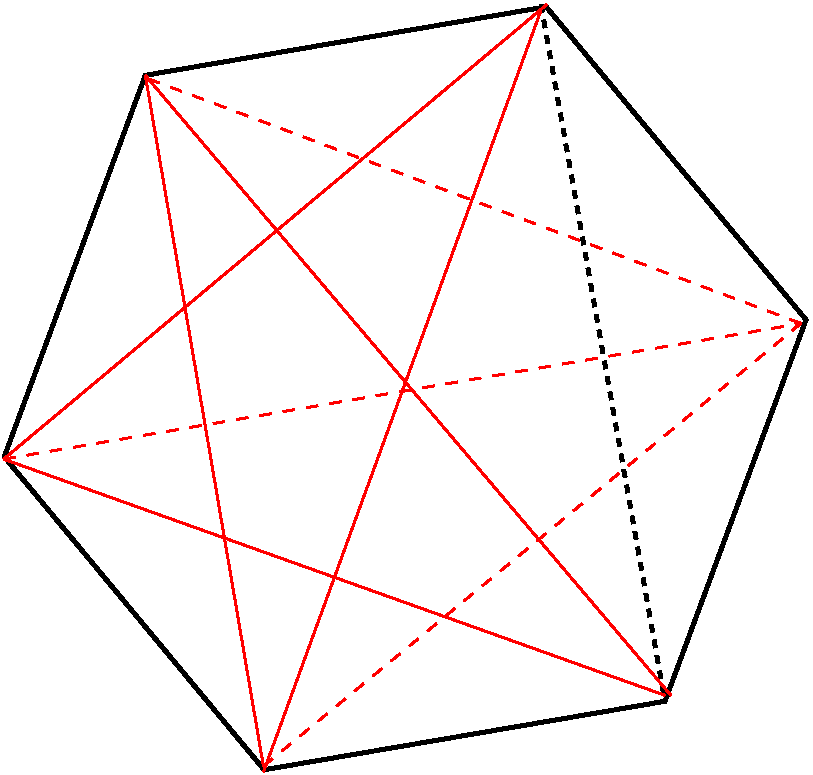
\includegraphics[width=6cm]{pictures/kulmiot}
\end{center}

%(kuvio kun 5-kulmiosta täydennetään 6-kulmio)

Siten $(k + 1)$-sivuisen monikulmion lävistäjien lukumäärä on
\[
\frac{k (k - 3)}{2} +k-1=
\frac{k (k - 3)}{2} + \frac{2k - 2}{2}
=
\frac{k (k - 3)+2k-2}{2}=\frac{k^2-k-2}{2}.
\]
Polynomilla $k^2 - k - 2$ on nollakohdat $k = -1$ ja $k = 2$. Polynomi tekijöihinsä jaettuna
on $k^2 -k -2 = (k + 1)(k- 2)$. Siis $(k + 1)$-sivuisen monikulmion lävistäjien lukumäärä
\[
\frac{(k + 1)(k - 2)}{2}= \frac{(k + 1)((k + 1)-3)}{2}.
\]
Kaava pätee siis myös kuperille $(k + 1)$-sivuiselle monikulmiolle.

Induktioperiaatteen nojalla kaava on tosi, kun $n=3,4,5,\ldots$.
\end{esimerkki}


\Harjoitustehtavat
%\newpage



%\section*{Tehtäviä.}

\begin{enumerate}

\item Osoita induktiolla, että luku $n^2+n$ on jaollinen luvulla $2$, kun $n$ on luonnollinen luku.

\item Osoita induktiolla, että luku $n^3+2n$ on jaollinen luvulla $3$, kun $n$ on luonnollinen luku.

\item Osoita induktiolla, että $2^n > n$, kun $n$ on positiivinen kokonaisluku.

\item Osoita induktiolla, että $n^2 > 2n + 1$, kun $n$ on kokonaisluku ja $n \ge 3$.

\item Osoita, induktiolla, että luku $7^n + 5$ on jaollinen luvulla $6$, kun $n$ on positiivinen kokonaisluku.

\item Osoita induktiolla, että luku $10^n - 3^n$ on jaollinen luvulla $7$, kun $n$ on positiivinen kokonaisluku.

\item Osoita induktiolla, että luku $7^n - 6n + 8$ on jaollinen luvulla $9$, kun $n$ on positiivinen kokonaisluku.

\item Osoita induktiolla, että $n! > n^2$, kun $n$ on kokonaisluku ja $n \ge 4$. Merkintä $n!$ tarkoittaa luvun $n$ \termi{kertoma}{kertomaa}. Se on tulo $n! = n \cdot (n-1) \cdot (n-2) \cdot \ldots \cdot 3 \cdot 2 \cdot 1$.

\item Olkoot $n$ positiivinen kokonaisluku ja $r$ reaaliluku, jolle pätee $r \neq 1$. Osoita induktiolla, että 
\[
1 + r + r^2 + r^3 + \ldots + r^{n-1} = \frac{1-r^n}{1-r}.
\]

\item Olkoon $n$ positiivinen kokonaisluku. Osoita induktiolla, että 
\[
1 \cdot 1! + 2 \cdot 2! + 3 \cdot 3! + \ldots + n \cdot n! = (n + 1)! - 1.
\]

\item 
Osoita induktiolla, että 
\[
\sum_{m=1}^n m^2= \frac{n(n+1)(2n+1)}{6}, \textrm{ kun } n=1,2,\ldots.
\]

\item
Osoita induktiolla, että $n$-alkioisessa joukossa on
\[
\frac{n(n-1)}{2}
\]
kahden alkion osajoukkoa, kun $n \ge 2$.

\item Todista kappaleessa 5.2 esiteltyjen kongruenssin laskusääntöjä koskevan lauseen kohta 4: Olkoot $a, b \in \Z$ ja $k,n \in \Z_+$ sekä $a \equiv b\ (\mod k)$. Tällöin $a^n \equiv b^n\ (\mod k)$.

\item Tarkastellaan kuviojonoa, joka muodostuu säännöllisen kuusikulmion muotoisista pistejoukoista. Jonon neljä ensimmäistä kuviota ovat seuraavat:

\begin{center}
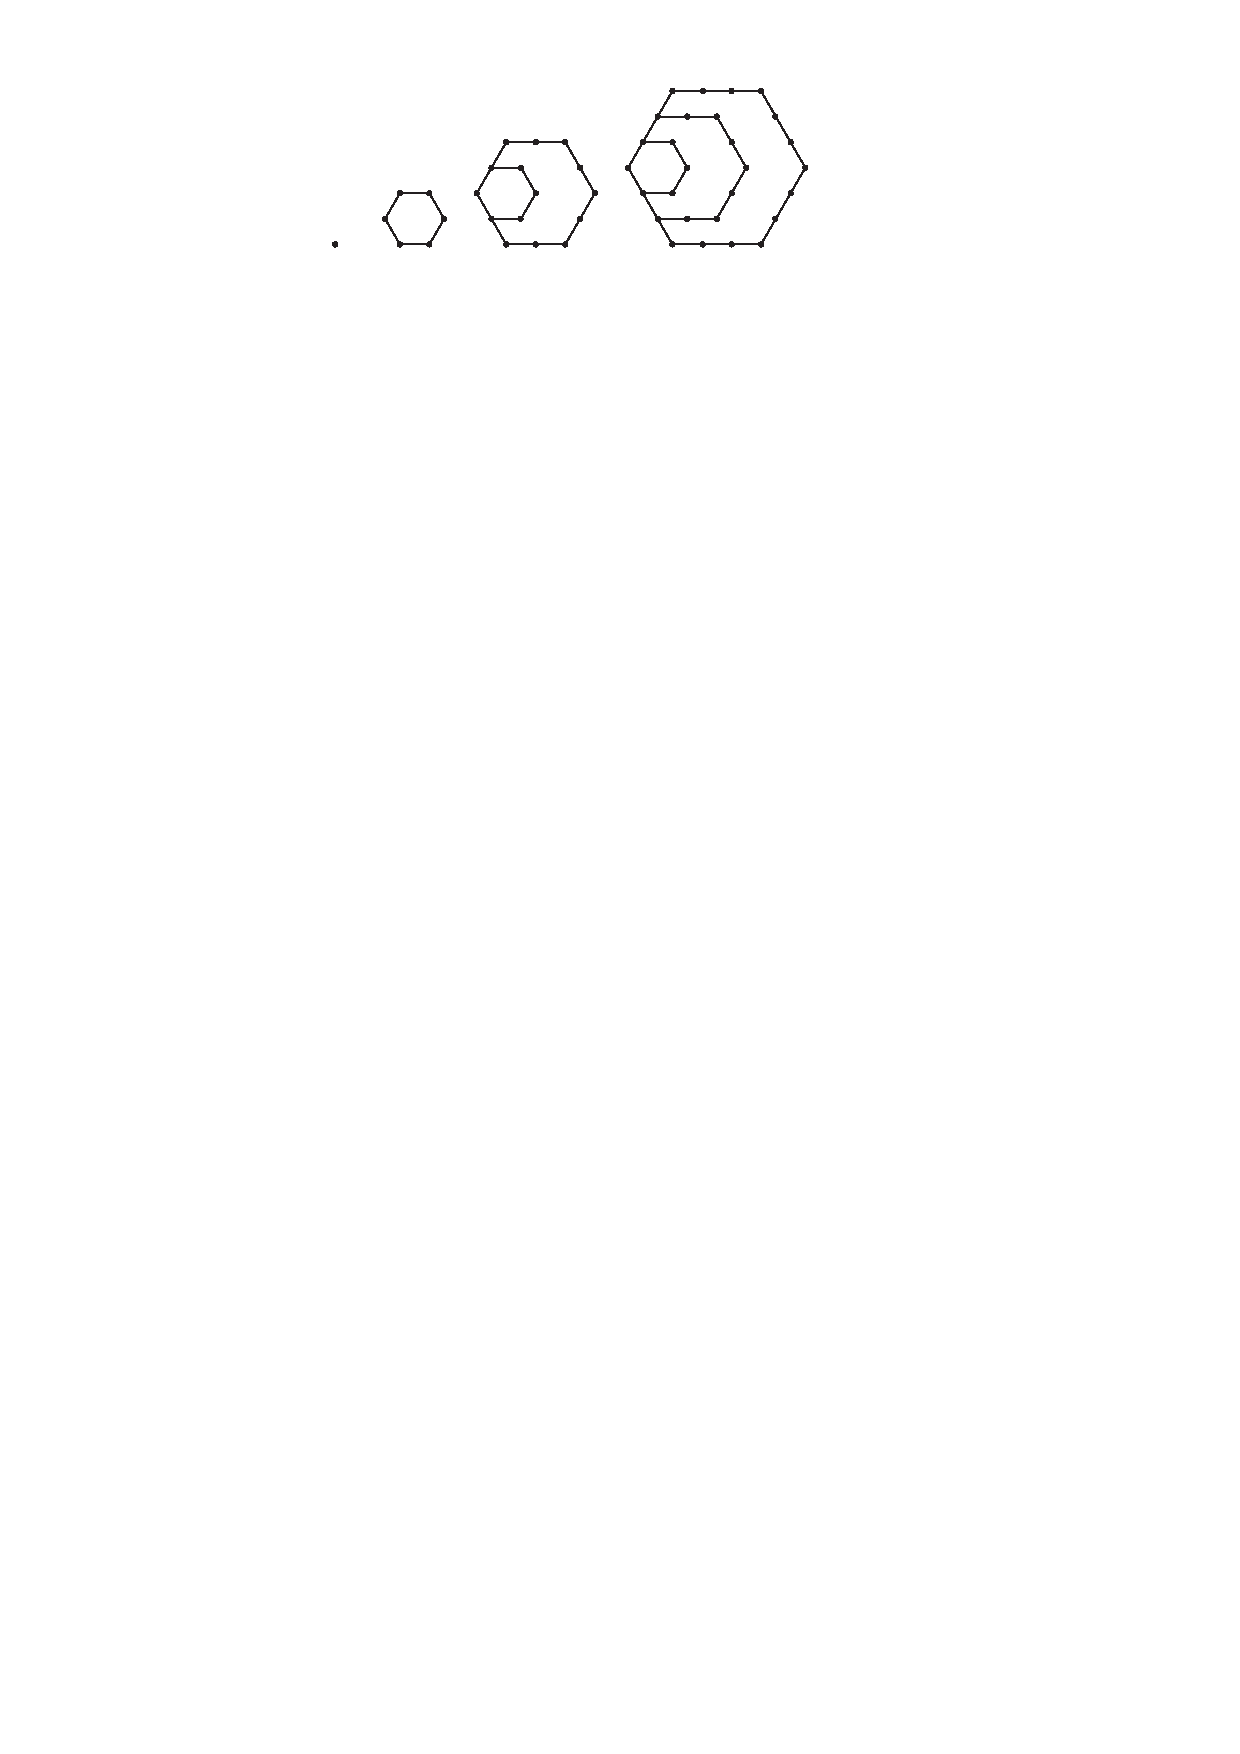
\includegraphics[width=10cm]{pictures/Kappale5_4_kuusikulm_v2}
\end{center}


\begin{itemize}
\item[a)] Laske, kuinka monta pistettä on kuviojonon kussakin neljässä ensimmäisessä kuviossa.
\item[b)] Muodosta kaava, jolla voidaan laskea, kuinka monta pistettä on $n$. kuviossa. Tarpeen vaatiessa voit hyödyntää laskimesi polynomisovitustoimintoja.
\item[c)] Todista kaava induktiolla.
\end{itemize}

\end{enumerate}

\subsection*{Kotitehtäviä}

\begin{enumerate}

\item Osoita induktiolla, että $n$ jakopisteellä jana voidaan jakaa enintään $n + 1$ janaksi.

\begin{center}
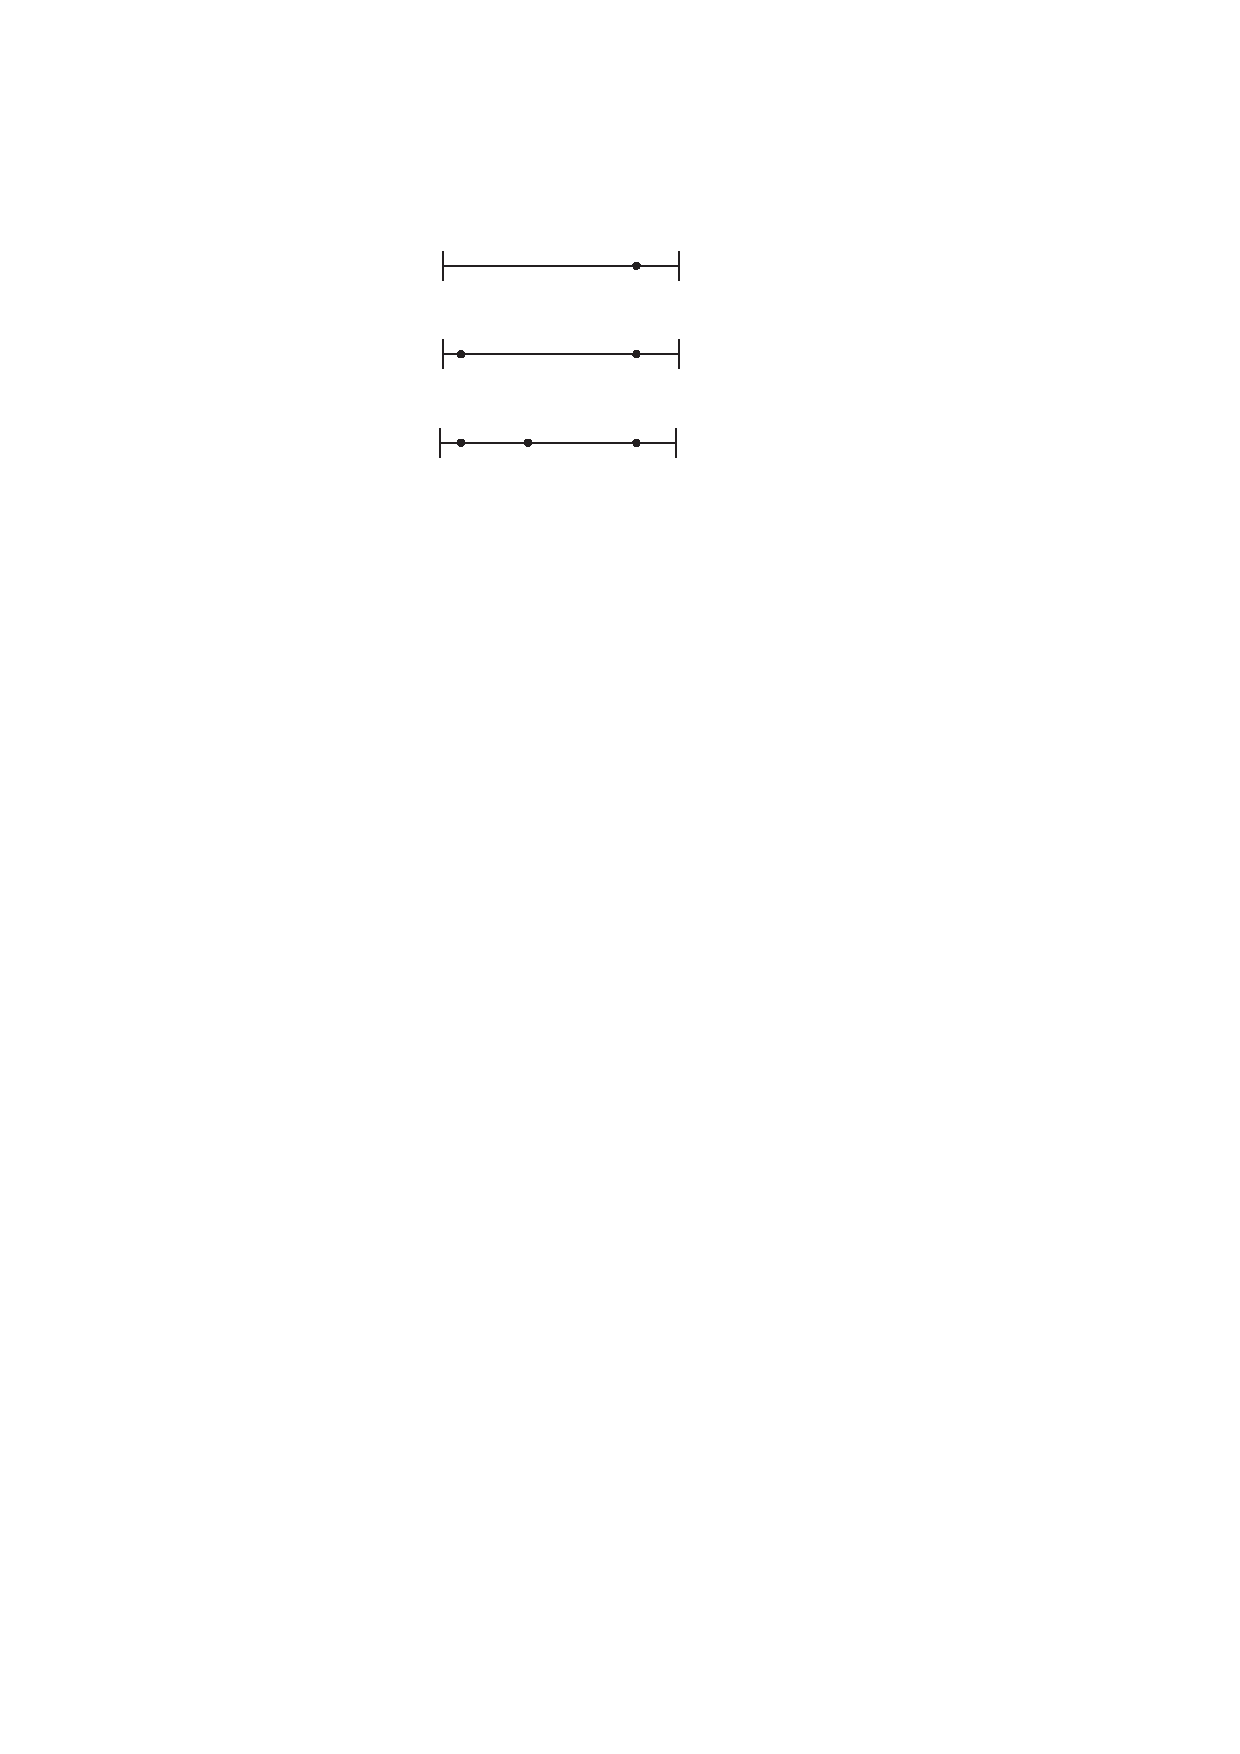
\includegraphics[width=6cm]{pictures/Kappale5_4_janat_v2}
\end{center}

\item Osoita induktiolla, että luku $n^3 + 5n$ on jaollinen luvulla $6$, kun $n$ on luonnollinen luku.

\item Osoita, että $3^n > 2n$, kun $n$ on positiivinen kokonaisluku.

\item Osoita induktiolla, että $3^n < n!$, kun $n$ on kokonaisluku ja $n\ge 7$.

\item Osoita induktiolla, että luku $6^n - 1$ on jaollinen luvulla $5$, kun $n$ on positiivinen kokonaisluku.

\item Osoita induktiolla, että luku $8^n - 5^n$ on jaollinen luvulla $3$, kun $n$ on positiivinen kokonaisluku.

\item Osoita induktiolla, että luku $27^{2n} + 3 \cdot 13^{n}$ on jaollinen luvulla $4$, kun $n$ on positiivinen kokonaisluku.

\item 
Osoita induktiolla, että
\[
\sum_{m=1}^n m^3= \frac{n^2(n+1)^2}{4}, \textrm{ kun } n=1,2,\ldots.
\]

\item Osoita induktiolla, että $(1 + 2 + 3 +\ldots + n)^2 = 1^3 + 2^3 + 3^3 + \ldots + n^3$, kun $n$ on positiivinen kokonaisluku.

\item Tasoon piirretään $n$ suoraa ($n\ge 2$). Osoita, että suorilla voi olla korkeintaan $n(n - 1)/2$ leikkauspistettä.

\item Tarkastele seuraavia luvun $2$ peräkkäisistä potensseista muodostuvia summia:
\[
\begin{array}{rcl}
1 &=& 1\\
1 + 2 &=& 3\\
1 + 2 + 4 &=& 7\\
1 + 2 + 4 + 8 &=& 15\\
1 + 2 + 4 + 8 + 16 &=& 31\\
1 + 2 + 4 + 8 + 16 + 32 &=& 63\\
1 + 2 + 4 + 8 + 16 + 32 + 64 &=& 127.
\end{array}
\]
Muodosta kaava, jolla voidaan laskea summa $2^0 + 2^1 + 2^2 + \ldots + 2^n$, missä $n$ on luonnollinen luku. Todista kaava induktiolla.

\item Olkoot $n$ luonnollinen luku ja $x$ reaaliluku, jolle pätee $x > -1$. Osoita, että $(1 + x)^n \ge 1 + nx$. Kyseessä on niin sanottu \termi{Bernoullin epäyhtälö}{Bernoullin epäyhtälö}.

\item Olkoon $n$ positiivinen kokonaisluku. Todista, että
\[
\frac{1}{2}\le\frac{1}{n+1}+\frac{1}{n+2}+\ldots +\frac{1}{n+n} <1.
\]
[YO syksy 1971 tehtävä 7]


\item
Osoita, että kaikilla positiivisilla kokonaisluvuilla $n$ on
\[
1^2+3^2+5^2+\ldots+(2n-1)^2 = \frac{n(4n^2-1)}{3}. 
\]
[Ylioppilastehtävä K98 8b]

\item Tarkastellaan ruudukoista muodostuvaa kuviojonoa, jonka neljä ensimmäistä kuviota ovat seuraavat:

\begin{center}
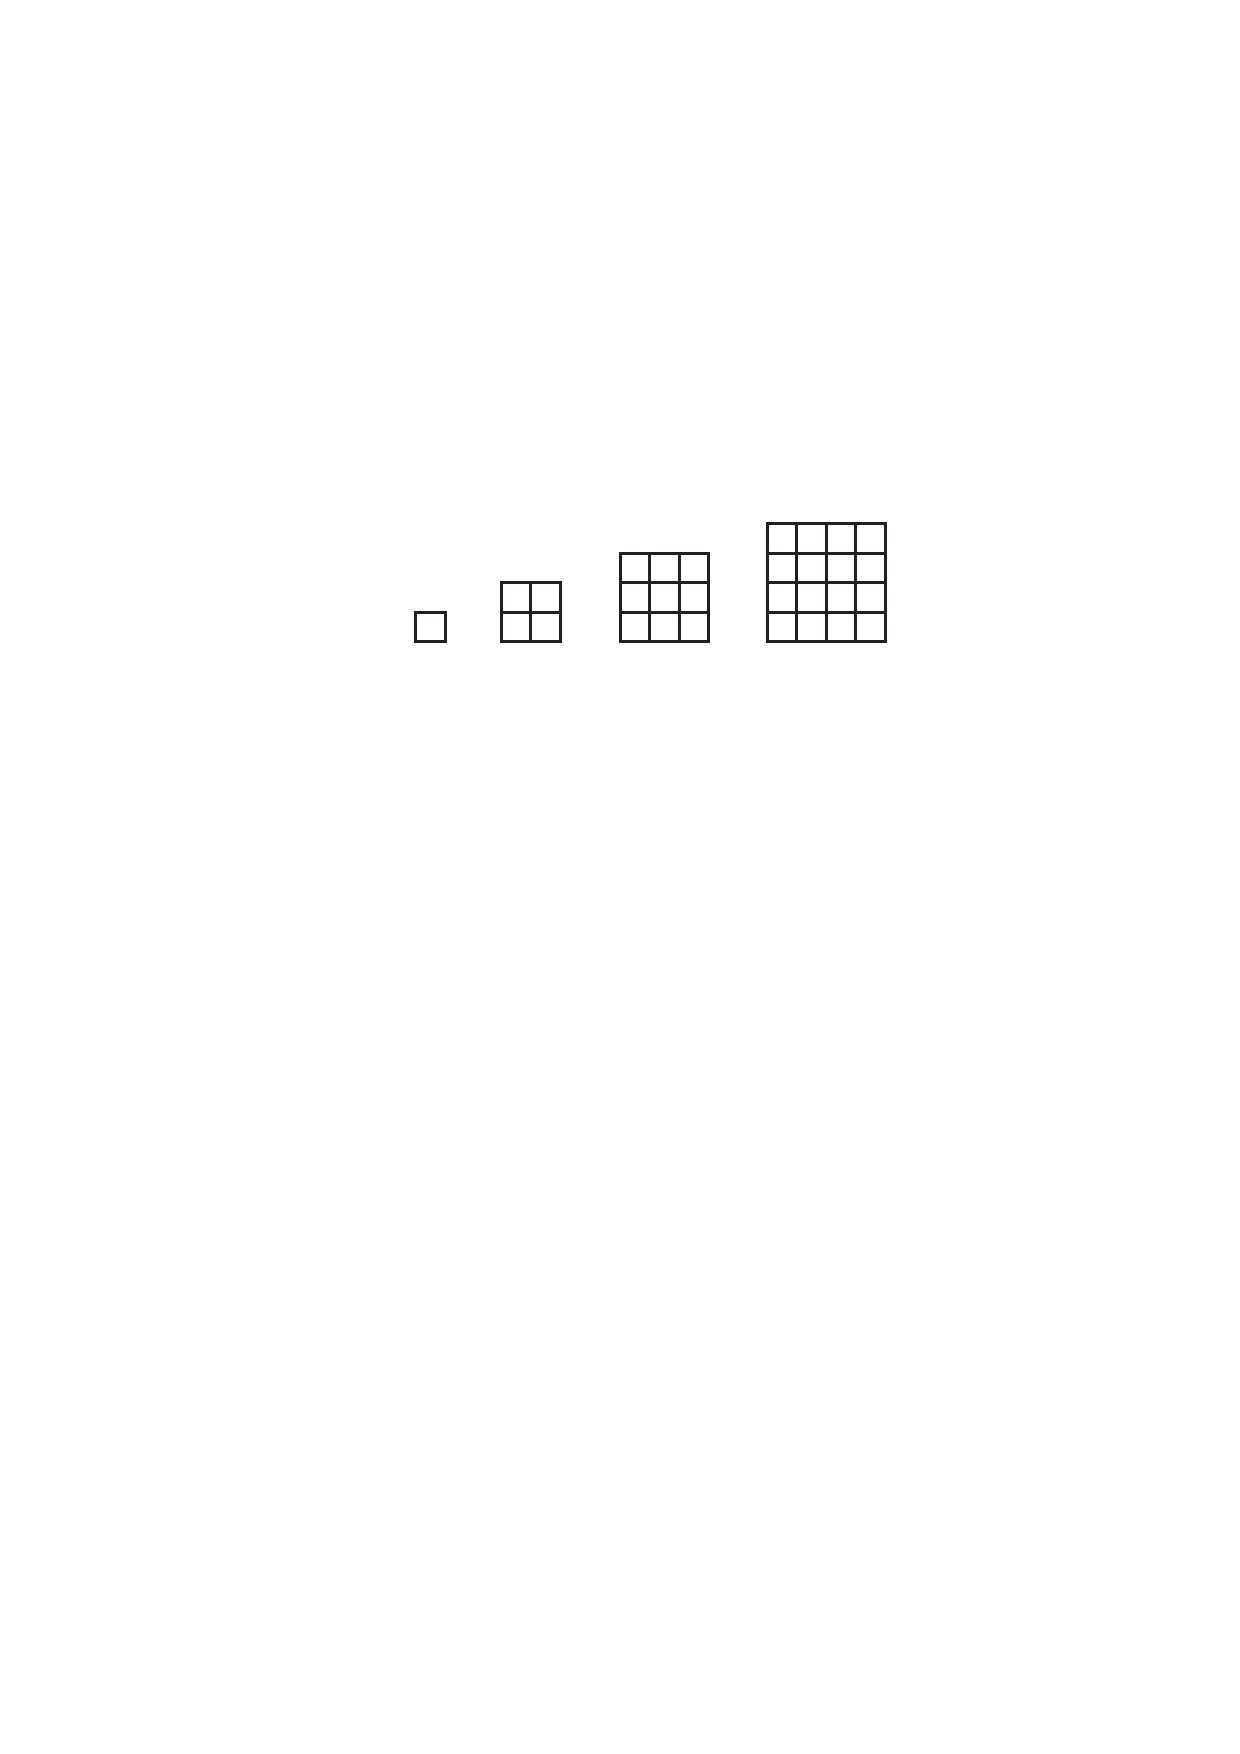
\includegraphics[width=10cm]{pictures/Kappale5_4_ruudukko_v2}
\end{center}

\begin{itemize}
\item[a)] Laske, kuinka monta neliötä kaikkiaan on kuviojonon kussakin neljässä ensimmäisessä ruudukossa.
\item[b)] Muodosta kaava, jolla voidaan laskea, kuinka monta neliötä on $n$. ruudukossa. Tarpeen vaatiessa voit hyödyntää laskimesi polynomisovitustoimintoja.
\item[c)] Todista kaava induktiolla.
\end{itemize}

\item Eräs keino, jolla voi tarkastaa onko yhteenlasku oikein suoritettu, perustuu seuraavaan lauselmaan:

Jos useampien kokonaislukujen summa ja samoin näiden lukujen numerosummien summa jaetaan yhdeksällä, niin tulevat jäännökset yhtä suuriksi. Todista tämä lauselma.
[YO 1895 tehtävä 2]


\end{enumerate}
